% ======================================================================
\documentclass[12pt,a4paper,oneside,openright]{book}

%───────── Auxiliary packages ──────────────────────────────────────────
\usepackage{blindtext}
\usepackage{mwe}
\usepackage{csquotes}
\usepackage{graphicx}
\usepackage{booktabs}
\usepackage{tabularx}
\usepackage{siunitx}
\usepackage{amsmath,amssymb}
\usepackage{algorithm}
\usepackage{algpseudocode}
\usepackage{listings}
\usepackage{nomencl}
\setcounter{tocdepth}{3}
\newcommand{\N}{\mathbb{N}}
\newcommand{\Z}{\mathbb{Z}}
\newcommand{\Q}{\mathbb{Q}}
\newcommand{\R}{\mathbb{R}}
\newcommand{\C}{\mathbb{C}}
\makenomenclature
\usepackage[
  backend=biber,
  style=numeric,
  sorting=nyt
]{biblatex}
\addbibresource{references.bib}

% Listings config
\lstset{
  basicstyle=\ttfamily\small,
  numbers=left,
  numberstyle=\tiny,
  columns=fullflexible,
  frame=single,
  breaklines=true,
  tabsize=2
}

\graphicspath{ {./images/} }

%───────── Template, covers, back cover ────────────────────────────────
\usepackage{template/sty_files/template-TFGspanish-uma}

\usepackage{template/sty_files/cotutor_cover-blueuma}
\usepackage{template/sty_files/cotutor_cover-whiteuma}

\usepackage{template/sty_files/backcover-uma}

%======================================================================
\begin{document}

%────────────────────── Blue front cover (Cotutor) ───────────────────────

\MakeBlueUMACover{
  degree     = {Grado en Ingeniería del Software},
  titleES    = {Recreación de exámenes psicotécnicos de conducción},
  titleEN    = {Recreation of psychotechnical driving exams},
  author     = {Pablo Luis Molina Blanes},
  tutor      = {Cristian Martín Fernández},
  cotutor= {Daniel Garrido Márquez},
  dept       = {Departamento de Lenguajes y Ciencias de la Computación},
  cityDate   = {Málaga, Junio, 2026},
  logoLeft   = {template/logos/NEG-uma-logo.png},
  logoRight  = {template/logos/NEG-etsi-logo.png}
}

%────────────────────── White front cover (Cotutor) ───────────────────────
\MakeWhiteUMACover{
  degree     = {Grado en Ingeniería del Software},
  titleES    = {Recreación de exámenes psicotécnicos de conducción},
  titleEN    = {Recreation of psychotechnical driving exams},
  author     = {Pablo Luis Molina Blanes},
  tutor      = {Cristian Martín Fernández},
  cotutor= {Daniel Garrido Márquez},
  dept       = {Departamento de Lenguajes y Ciencias de la Computación},
  cityDate   = {Málaga, Junio, 2026},
  defenseDate = {Julio, 2026},
  logoLeft   = {template/logos/POS-uma-logo.png},
  logoRight  = {template/logos/POS-etsi-logo.png}
}

\frontmatter

%────────────────────── Abstracts ──────────────────────────────────────
\renewcommand{\abstractname}{Resumen}


%──────────────── Acknowledgments ───────────────────────────────────────
\begin{umaacknowledgments}
Agradezco a los tutores académicos su constante colaboración, apoyo y preocupación conforme estuve desarrollando este proyecto. 

Agradezco también el apoyo incondicional en términos económicos y emocionales de mi familia. 

Me gustaría agradecer también a todos los creadores de contenido tecnológico que existen en Internet, es un trabajo poco apreciado y que se da demasiado por sentado en la sociedad; sin ellos, este trabajo no podría haber sido posible. 
\end{umaacknowledgments}

%────────────────────── TOC and lists ──────────────────────────────────
\clearpage
\tableofcontents
\clearpage
\listoffigures
\clearpage
\listoftables
\clearpage

%────────────────────── Nomenclature ───────────────────────────────────

\clearpage

\mainmatter
%────────────────────── Chapter 1 — Introducción ───────────────────────
\chapter{Introducción}

FOSS Psychotechnical Examination busca ser una recreación, en forma de software libre y abierto, de una suite software de evaluación psicotécnica para conductores.

Dispone de componentes software para sistemas empotrados, de software de sistemas, y de software de aplicación.

Tradicionalmente, las suites software ya existentes para este tipo de uso, como por ejemplo, la proporcionada por General ASDE o LN Deter se ofrecen bajo servicios cerrados a clínicas; esto no permite estudiar su funcionamiento, ni mucho menos modificarlo o construir sobre estos productos.

La recreación no se suele considerar habitualmente como 'innovación', y no se valora como esfuerzo original y propio en muchos campos; pero es gracias a la recreación que podemos conocer cuándo una técnica funciona de forma consistente, y podemos establecer qué es lo que funciona, y lo que no.

Con las nuevas tecnologías y buenas prácticas de las que disponemos, es especialmente importante esta replicación, nos permite desarrollar sobre las fórmulas que ya funcionaron en el pasado, y obtener nuevo conocimiento gracias a esta tarea de adaptación a un mundo distinto. 

\section{Descripción por capítulo}

\subsection{Marco teórico}

En el marco teórico se expone y se describe y se acreditan los temas, campos del saber, y técnicas más relevantes y utilizadas para FOSS Psychotechnical Examination.

Aquí se introduce una colección de técnicas matemáticas, psicológicas y de desarrollo software; además del contexto legal y social de herramientas de evaluación psicotécnica.

\subsection{Análisis}

En la sección de análisis nos introducimos a las funcionalidades de cada componente de FOSS Psychotechnical Examination. Busca ser una colección resumida de las funcionalidades más importantes para el correcto funcionamiento del suite software.

\subsection{Diseño}

En esta sección se expone la arquitectura de la suite software en general; y de todos sus componentes individuales. También se entra en detalle en la arquitectura y decisiones relativa a hardware y dispositivos electrónicos utilizados en el proyecto.

\subsection{Implementación}

En esta sección se describen y desarrollan los flujos de ejecución principales de la aplicación, desarrollados paso a paso y con explicaciones varias.

\subsection{Funcionamiento}

En esta sección se introducen los roles que pueden tomar los usuarios de la aplicación; se han incluido roles tradicionales como el del usuario o el del doctor; y también se ha incluido aquí el rol de atacante para enfatizar posibles intentos de ataque, y protecciones otorgadas por la suite software ante estos ataques

\subsection{Pruebas}

Aquí se describen las tecnologías de pruebas que se han utilizado para cada componente de esta suite software; además de las pruebas realizadas, su razonamiento, y los resultados esperados.

\subsection{Conclusiones}

Aquí se da una recolección de lo aprendido y realizado en este proyecto; desde el ángulo de vista de la retrospectiva.

\subsection{Anexos}

Aquí se introducen documentos explicativos, que sirven para desarrollar aspectos no fácilmente desarrollables como secciones dentro del documento de la memoria; se incluye un manual de usuario, un manual de instalación, y un modelo de formulario de consentimiento para el tratamiento de los datos de usuarios.

%────────────────────── Chapter 2 — Marco teórico ───────────────────────
\chapter{Marco teórico}
\section{Estado del arte}

En el campo de los dispositivos para realizar test psicotécnicos a conductores, existen varios
aparatos que realizan esta funcionalidad.

\subsection{General ASDE}

Originalmente conocidos como \textit{ASDE-Operator} hasta convertirse en la llamada \textit{General ASDE} a finales de 1988\cite{commodorearticle}, es una empresa dedicada al diseño, fabricación y mantenimiento de Productos Sanitarios, inscrita ante la AEMPS (Agencia Española del Medicamento y el Producto Sanitario); sus productos más conocidos son aquellos relativos al Reconocimiento Médico y Psicotécnico.

Es una empresa con certificado ISO 9001, y desarrolla sus productos conforme a normativas europeas e internacionales; entre los que se incluye la Directiva Europea 93/42/CEE\cite{asde1}

Su principal producto relativo a realizar reconocimientos psicotécnicos es el denominado Asde Driver Test N-845; basado en el programa predecesor Driver-Test, entonces desarrollado por el equipo compuesto por el profesor de la UPV (Universidad Politécnica de Madrid) Dr. Héctor Monterde i Bort, junto con José Urnaga.\cite{asde2}

\subsection{LN Deter}


LN Deter es una empresa española especializada en diseño, desarrollo y fabricación de tecnología médica y soluciones telemáticas \cite{lndeter2}

El principal dispositivo de la compañía consiste en el LND-100 \cite{lndeter1}; el cual se comenzó a desarrollar por el propio fundador de la compañía, Fernando Ortiz, y un amigo suyo. Francisco Ortiz se iría después a Londres, y habría desarrollado su idea. \cite{lndeter3}



\section{Técnicas y fórmulas matemáticas}

\subsection{Detección de colisiones}

La detección de colisiones, al tratarse de una operación de una única dimensión, se realiza por medio de la siguiente operación matemática:

Siendo $x_c$ la posición en x del coche, $s_c$ la anchura en x del coche, $x_w$ la posición en x de la pared y $s_w$ la anchura en x de la pared, se calcula si se ha producido una colisión de la siguiente forma

$f(x_c,x_w,s_c,s_w) =$ $\begin{cases}0 & (x_c < x_w) \lor (x_c > x_w+(s_w-s_c))\\ 1 & (x_c \geq x_w) \lor (x_c \leq x_w+(s_w-s_c)) \end{cases}$

De ser el resultado 0, afirmamos que el vehículo se encuentra dentro de la pared; de ser el resultado 1, afirmamos que el vehículo se encuentra fuera de la pared.

\section{Criptografía}

La criptografía es un campo de las matemáticas aplicadas. Busca asegurar una comunicación segura contra adversarios.

\subsection{Funciones hash}

Son funciones que generan una entrada de tamaño variable, y devuelven una salida de tamaño fijo. Para que estas funciones sean seguras, debe ser resistente ante colisiones (es decir, dos valores que se resuelvan a la misma salida), y para la misma entrada, siempre se debe computar la misma salida.

\subsection{Encriptación en bloque}

Consiste esta en una modalidad de encriptado que devuelve un texto cifrado cifrándolo a lo largo de varios bloques. El texto sin descifrar entonces se dividiría en varios bloques, cada uno del tamaño de la clave, y se cifraría progresivamente repitiendo la misma clave para todos los bloques.

Para descifrar, sería cuestión de dividir el texto cifrado en bloques, y descifrar progresivamente haciendo la operación inversa con la clave.

Cuando la clave no se repite, y es de la misma longitud que el texto cifrado, estaríamos haciendo uso de una libreta de un solo uso.

Para este trabajo, en específico, se utiliza el cifrado AES-256.

Se pueden utilizar dos modalidades distintas:

\begin{enumerate}
  \item \textbf{Modalidad ECB}: La modalidad ECB consiste en utilizar la clave únicamente para realizar el encriptado. Es un modelo poco recomendado ya que un atacante puede obtener patrones a partir del texto cifrado.
  \item \textbf{Modalidad CBC}: La modalidad CBC añade el concepto de un vector de inicialización, que se genera de forma aleatoria, y que se utiliza para prevenir que un texto cifrado, para la misma entrada, sea siempre el mismo. Esto impide que un atacante pueda obtener información utilizando patrones del texto cifrado.
\end{enumerate}

\begin{figure}[H]
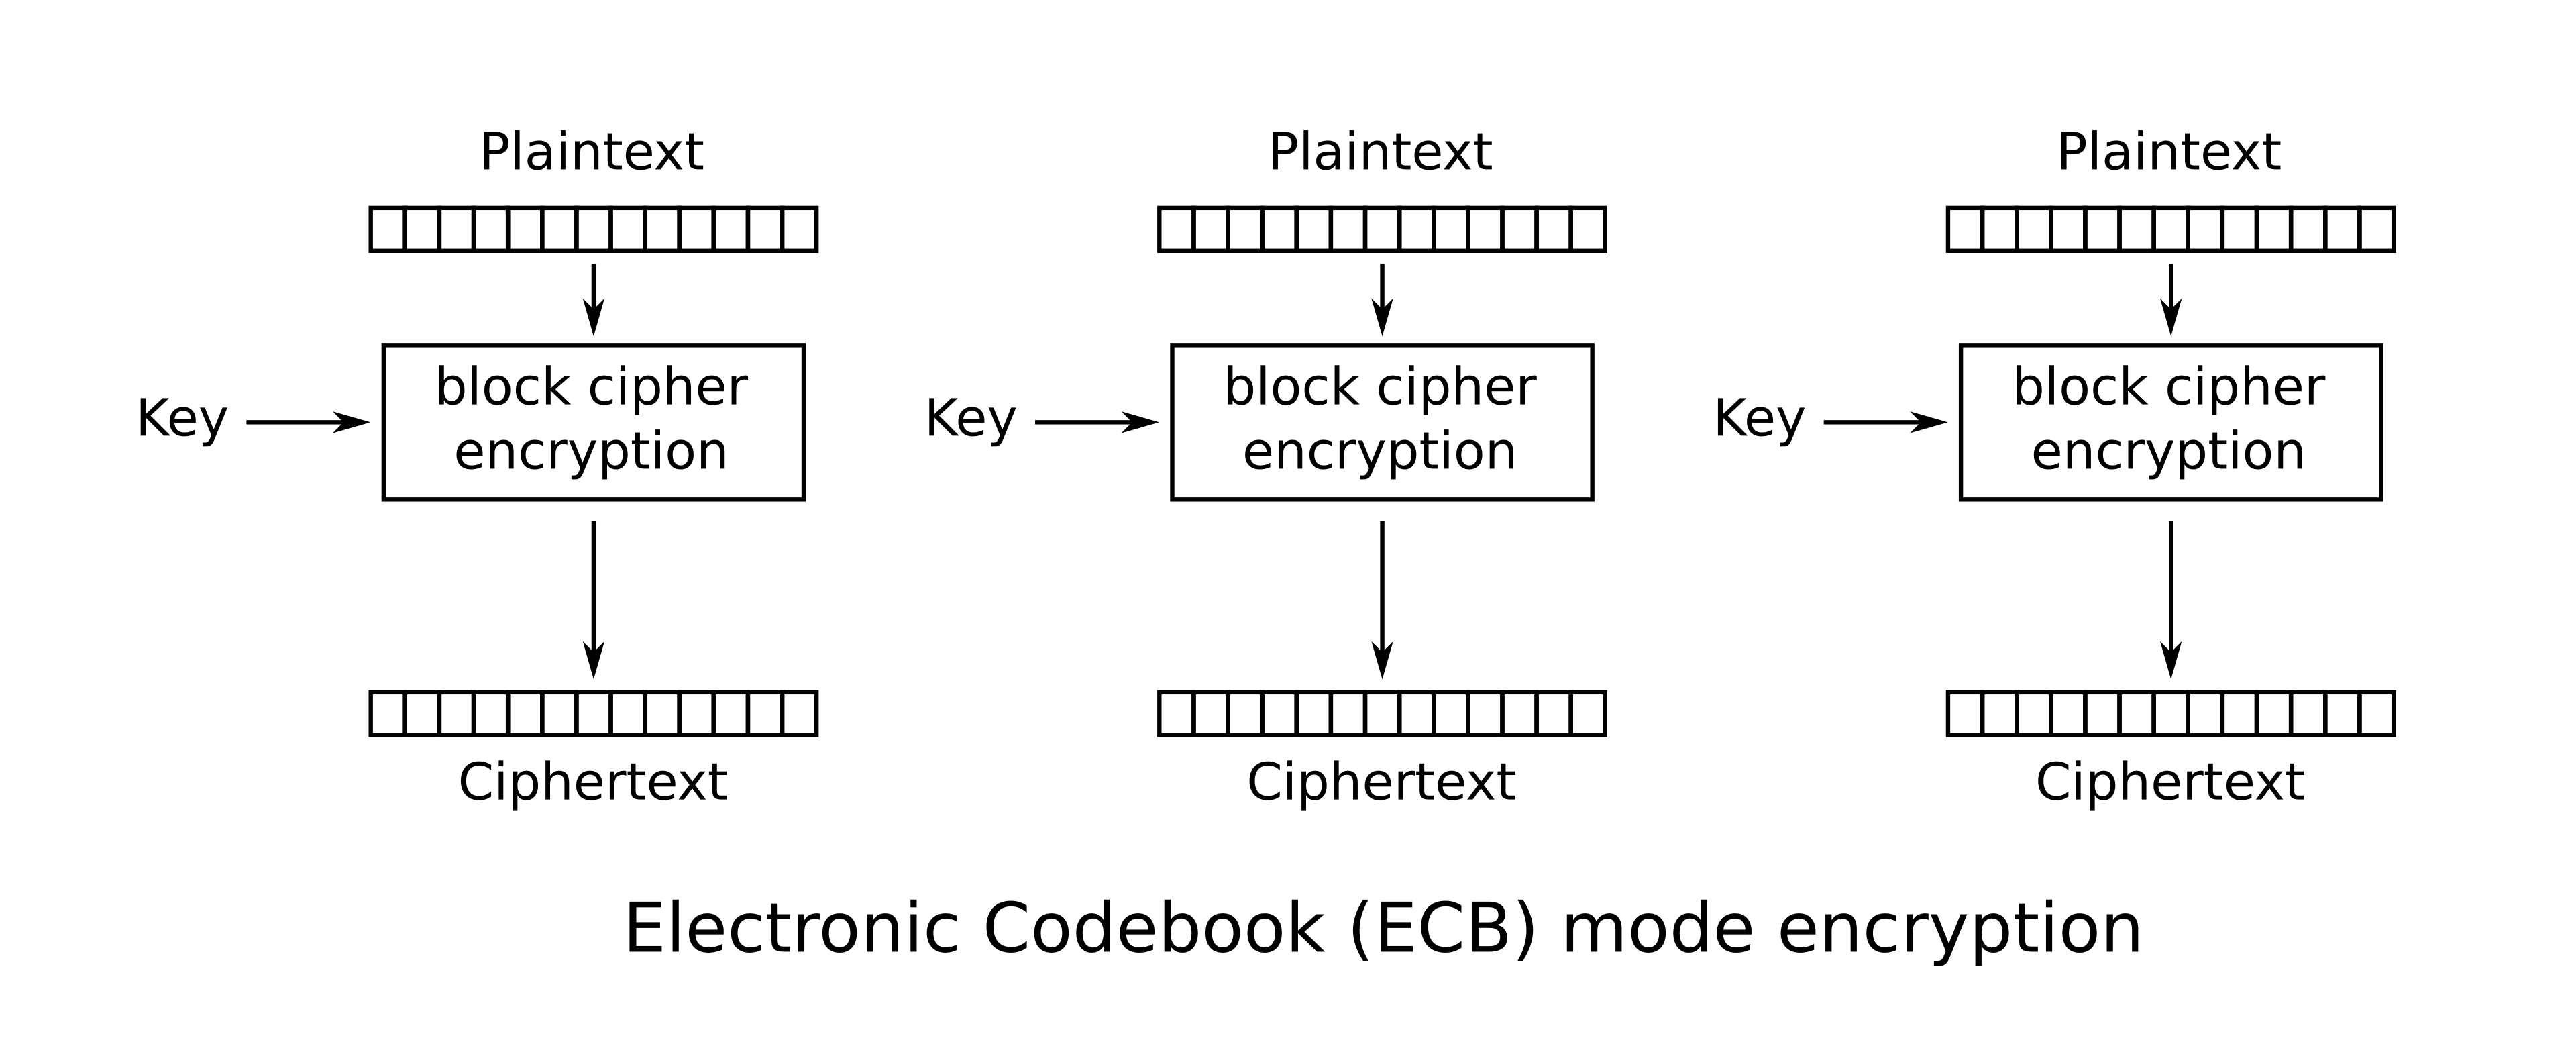
\includegraphics[width=1.1\textwidth]{ECB_encryption.svg.png}
\caption{Diagrama de encriptado ECB \cite{ecb1}}
\end{figure}
\begin{figure}[H]
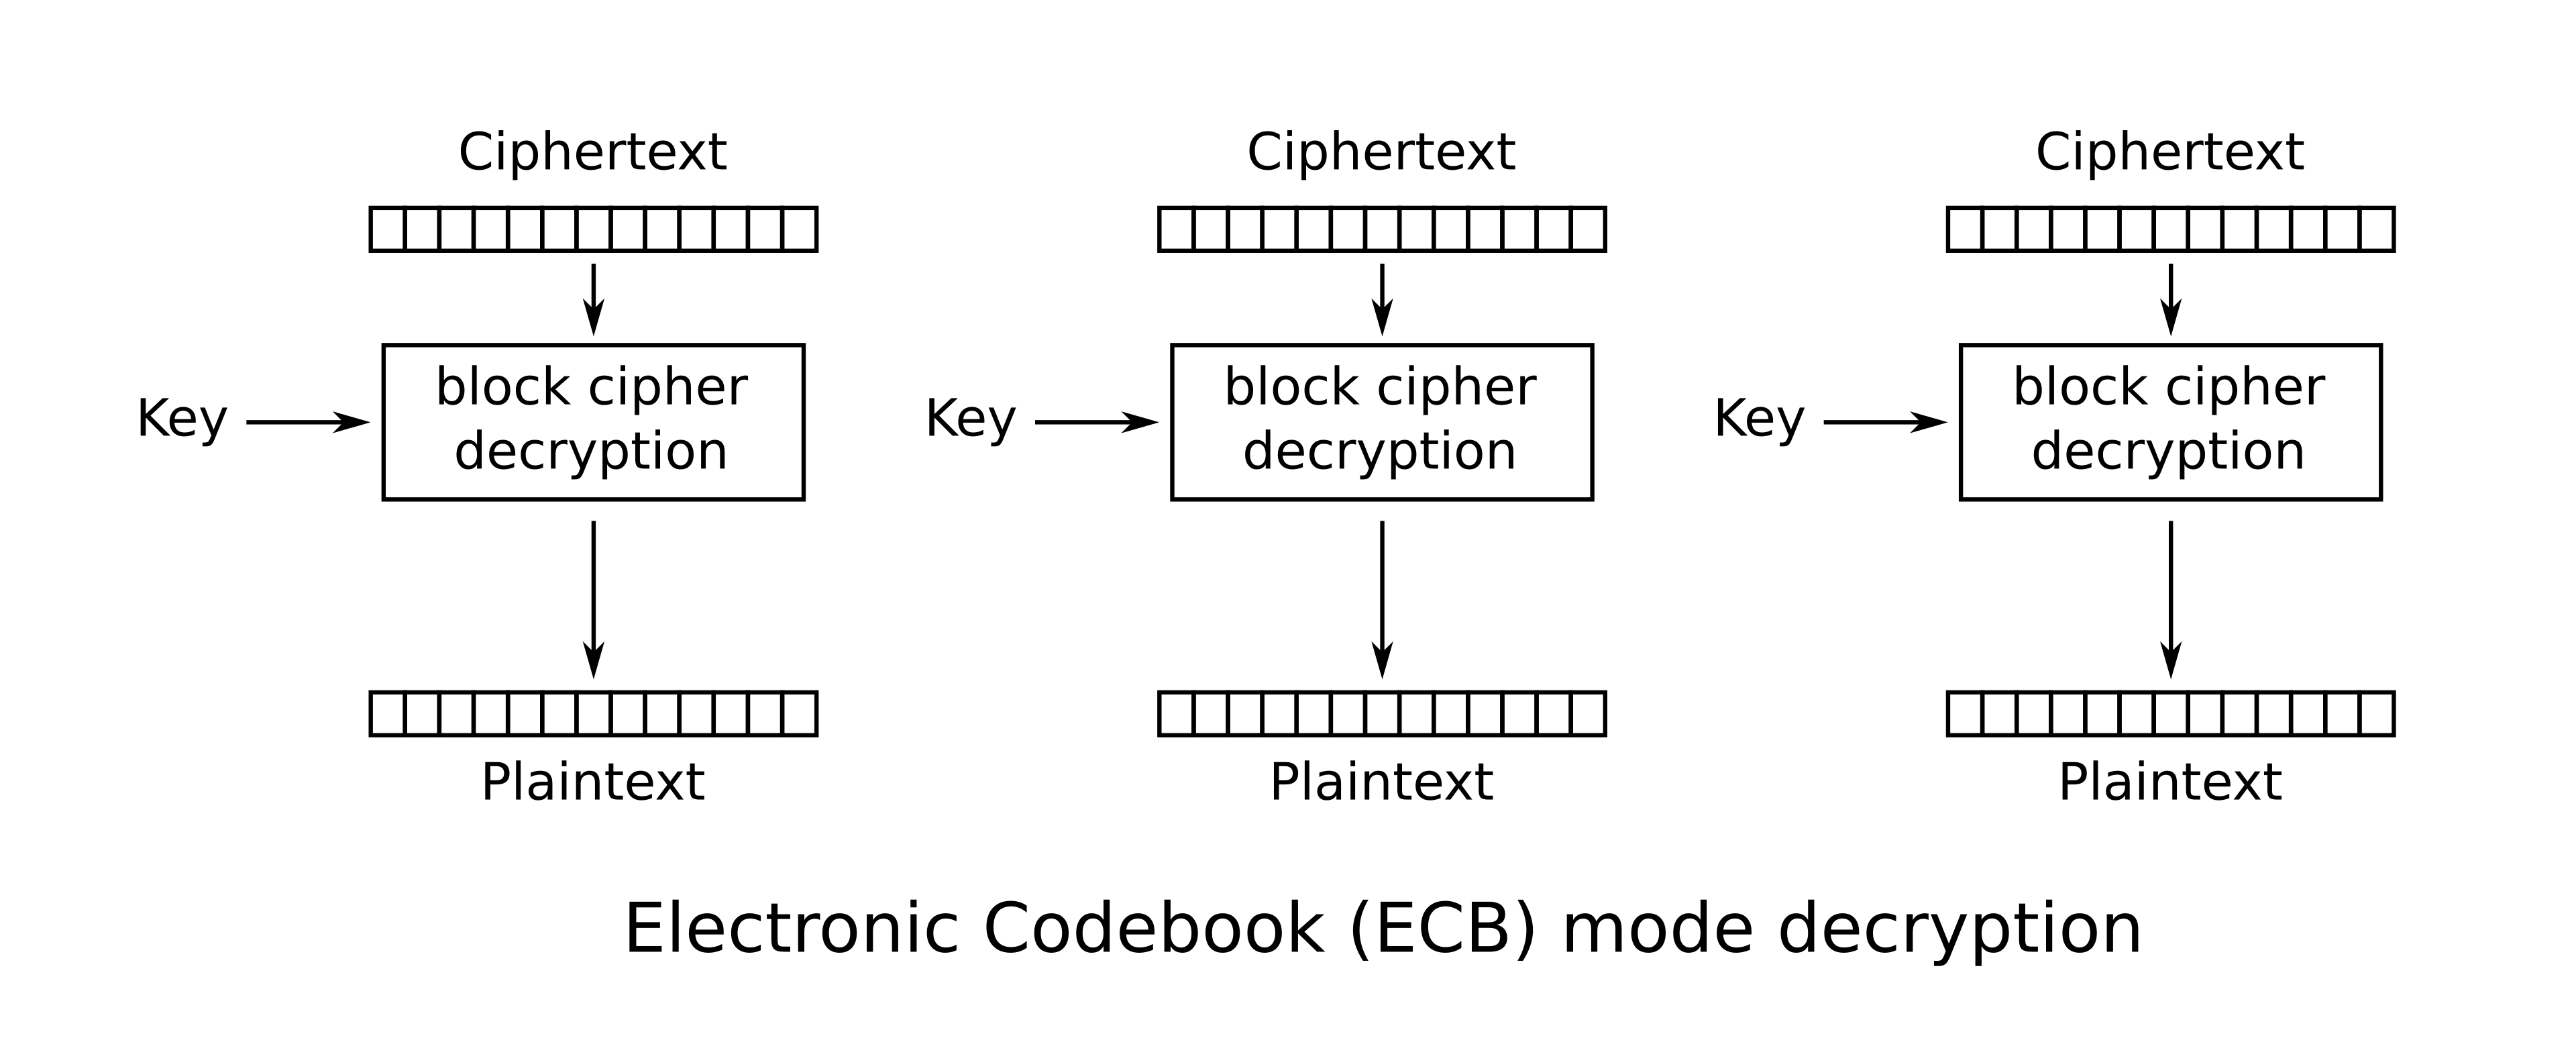
\includegraphics[width=1.1\textwidth]{ECB_decryption.svg.png}
\caption{Diagrama de desencriptado ECB \cite{ecb2}}
\end{figure}
\begin{figure}[H]
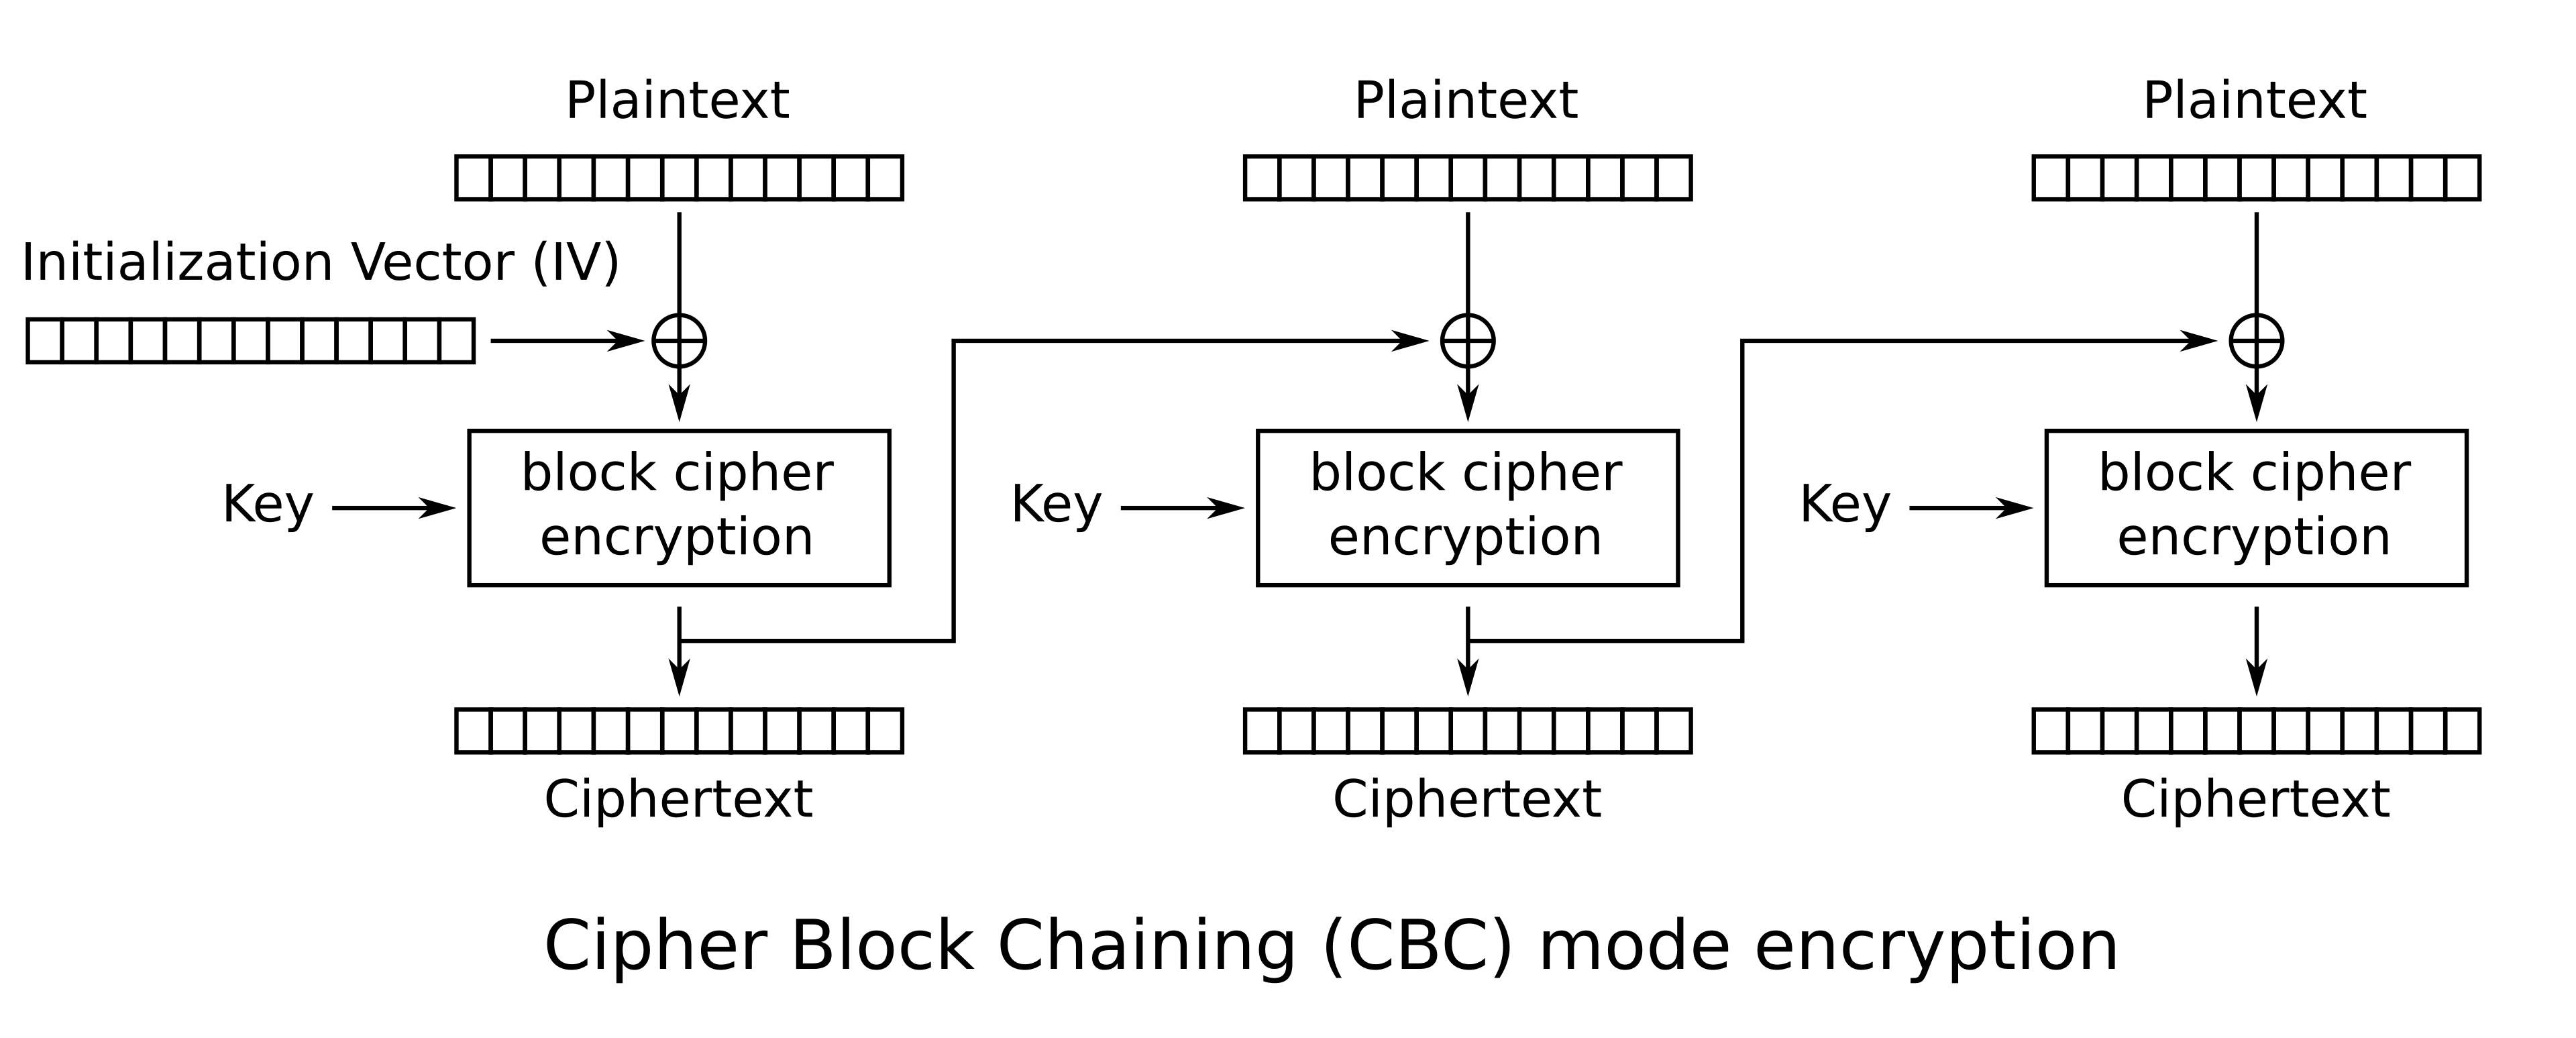
\includegraphics[width=1.1\textwidth]{CBC_encryption.svg.png}
\caption{Diagrama de encriptado CBC \cite{cbc1}}
\end{figure}
\begin{figure}[H]
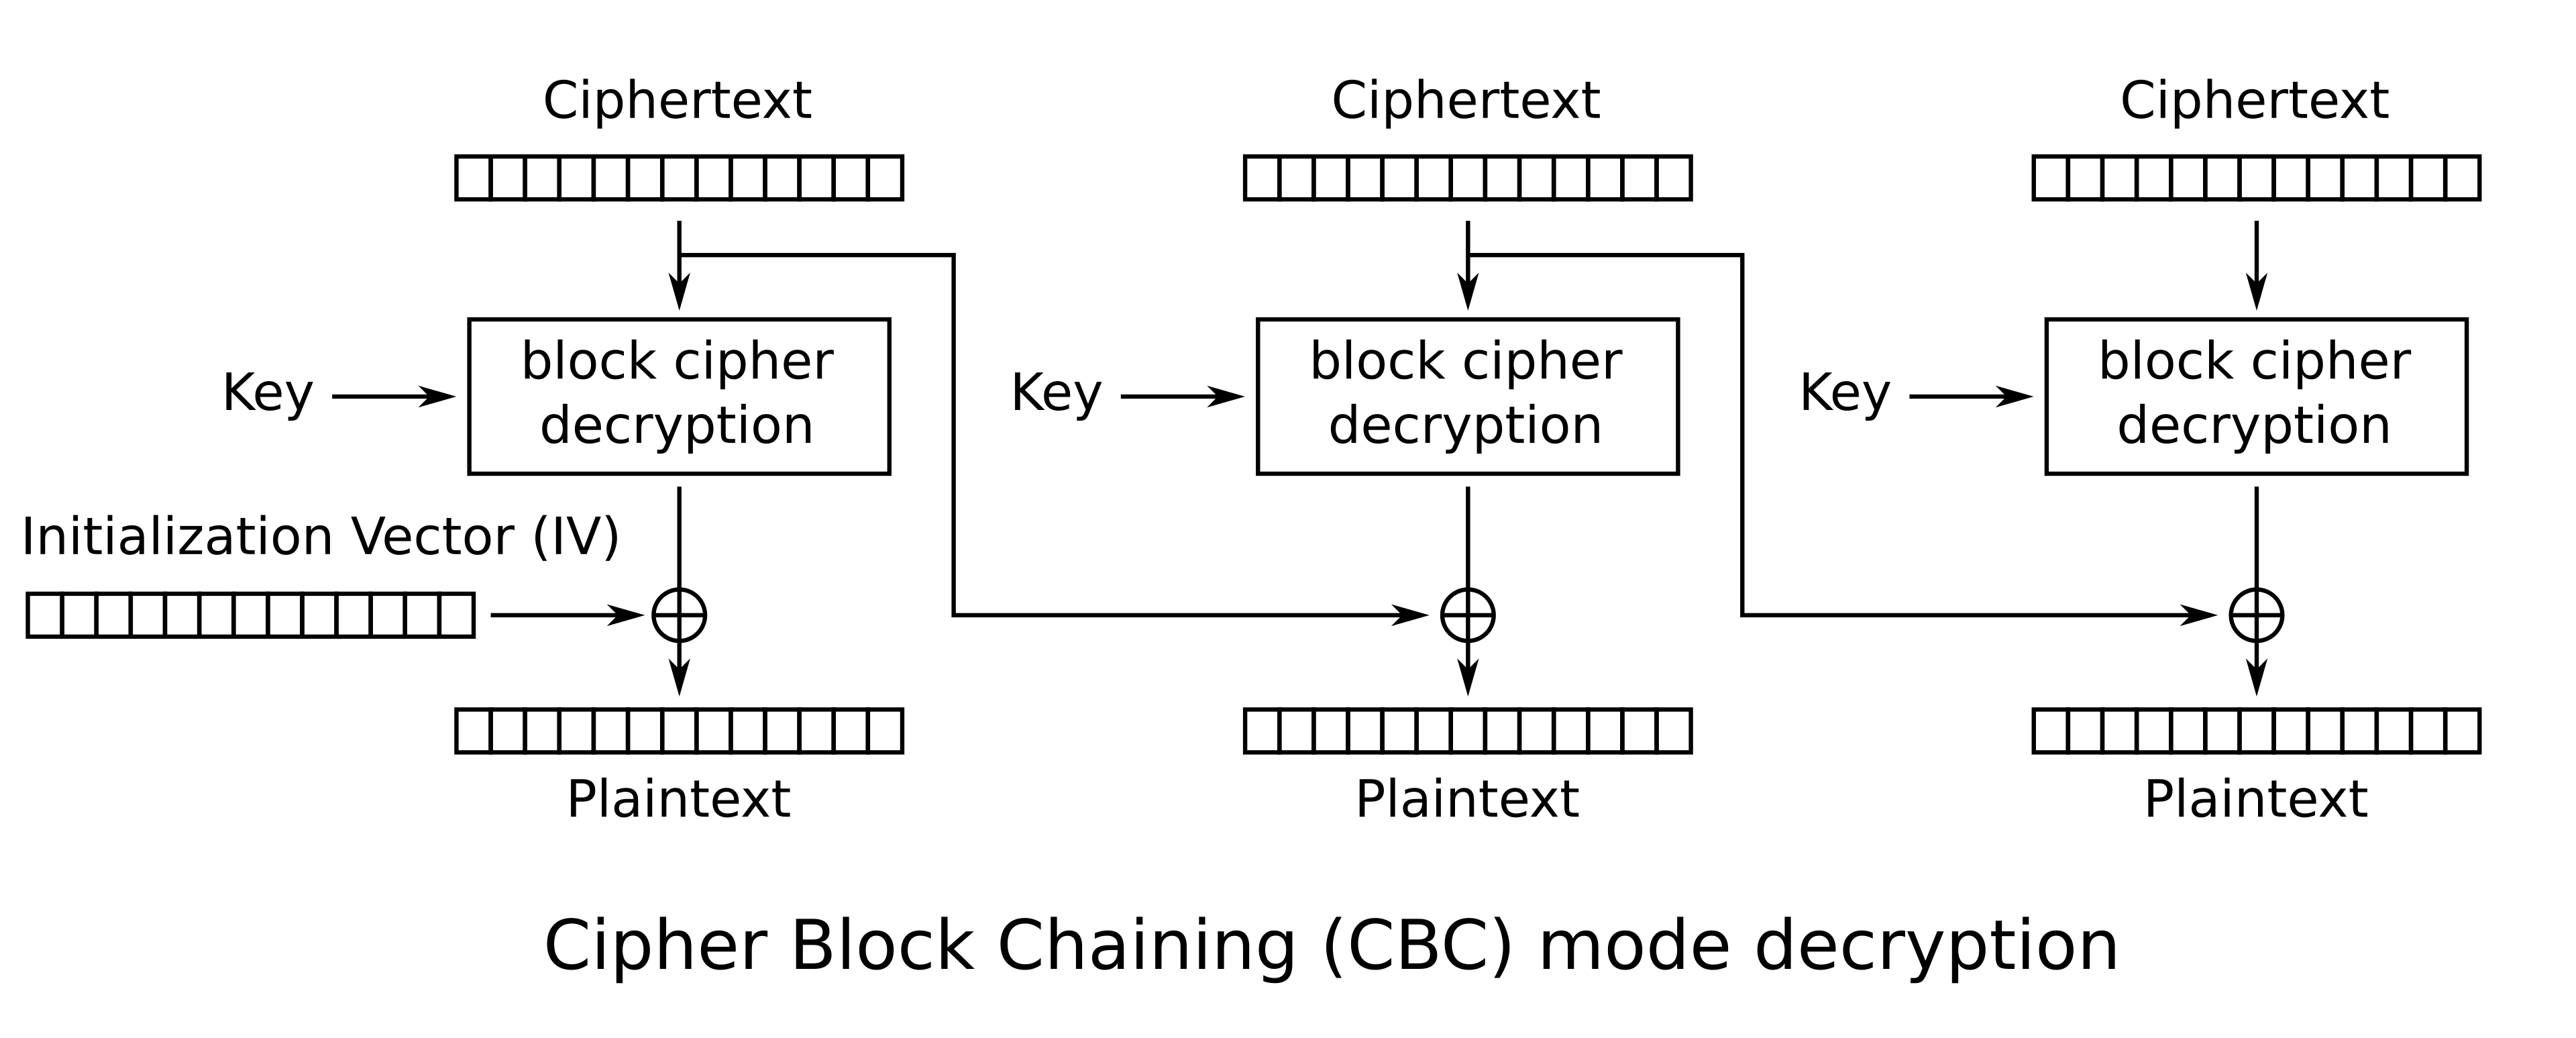
\includegraphics[width=1.1\textwidth]{CBC_decryption.svg.png}
\caption{Diagrama de desencriptado CBC \cite{cbc2}}
\end{figure}

\subsubsection{Cifrado AES}

El cifrado AES consiste en una variación del cifrado por bloques Rijndael, originalmente diseñado por Joan Daemen y Vincent Rijmen.

Se basa en una red de sustitución-permutación; donde se definen dos tipos de bloques, denominados S-boxes y P-boxes, que realizan varias iteraciones alternantes sobre una clave y un texto a cifrar; para devolver un texto cifrado.

\section{Técnicas y métricas cognitivo-psicológicas}

El campo de la psicología cognitiva proporciona a la comunidad científica un entendimiento, desde el punto de vista de la cognición, sobre cómo hacemos uso de nuestros recursos cerebrales en todo tipo de situaciones. Es un campo muy basado en los experimentos.

Este campo dispone de métricas y técnicas que resultan relevantes para asegurar una conducción segura en un contexto de conducción, que son ampliamente utilizadas en exámenes psicotécnicos. Aquí se detallan algunas definiciones importantes:

\subsection{Tiempo de reacción}

El tiempo de reacción se define por la DGT (Dirección General de Tráfico) como el tiempo que pasa entre que un peligro aparece, y un conductor se percata del peligro.

El tiempo estándar de un ser humano de reacción torna alrededor de unos 300 milisegundos.

\subsection{Velocidad de anticipación}

Se define como la capacidad de un sujeto para percibir velocidades y trayectorias, y su capacidad de autocontrol

El examen de tiempo de anticipación se desarrolla primero en el artículo científico de 1966. \cite{maruyama1966speed}

En este examen, se presentan dos objetos, un cuadrado blanco, y un túnel; el examinado deberá anticipar, al entrar el cuadrado blanco por un lado del túnel, cuándo saldrá por el otro lado de ese túnel.

Un tiempo demasiado bajo se considera impulsivo, mientras que un tiempo demasiado alto se considera falto en tiempo de reacción.

\subsection{Coordinación mano-ojo}

La coordinación mano-ojo, para un sujeto, consiste en su capacidad de traducir lo que percibe de forma visual, a movimientos específicos de su mano.

El examen de tiempo de anticipación se desarrolla primero en el libro de 1943. \cite{bonnardel1943adaptation}

En este examen, se hace uso de un dispositivo el cual muestra dos vehículos, controlados por dos manivelas; cada vehículo se puede accionar a la izquierda o a la derecha.

El objetivo del examinado consiste en mantener los dos vehículos dentro de sus respectivas carreteras, e impedir en la medida de lo posible que cualquiera de los dos vehículos se salga por demasiado tiempo; lo cual indicaría una falla en esta métrica.

\section{Legalidad y conformidad a la legislación Española y Europeas}

\subsection{Protección de Datos \cite{apuntesprotecciondatos}}

La Protección de los Datos es un campo legal con una larga historia.

En este campo se busca regular todo lo relativo al uso de los datos personales de individuos físicos.

Dentro del marco de este proyecto, es muy relevante esta regulación, ya que trabajamos con datos personales de individuos físicos directamente, y es importante tomar medidas organizativas y técnicas para prevenir el uso ilícito de estos datos.

En territorio Europeo, todo esto se regula bajo el Reglamento General de Protección de Datos; regulación que se implementa en los territorios nacionales de la Unión Europea.

\subsubsection{Reglamento General de Protección de Datos} \cite{EuropeanParliament2016a}

Reglamento con última versión datada el 4 de Mayo de 2016.

Busca proteger los datos de personas físicas, denominadas como *interesados* en el marco de esta legislación, obligando a los denominados *responsables* a tomar varias medidas por reglamento; se incluyen especificaciones de variada índole, entre las que se incluyen:
\begin{enumerate}
  \item Definiciones de datos personales y tipos de datos personales, junto con sus obligaciones
  \item Definición de la figura del responsable, del encargado, delegado, y del interesado en el marco de los datos personales
  \item Obligación de los responsables de informar a los interesados en sus derechos, en el tratamiento de sus datos, y en otras formas de información
  \item Obligación de los responsables a tomar medidas técnicas y organizativas para proteger los datos
\end{enumerate}

Se ha incluido, a modo de ejemplo, un modelo de documento de política de protección de datos a fin de ejemplificación sobre cómo se podría aplicar esta regulación a este proyecto.

\subsubsection{Ley Orgánica de Protección de Datos} \cite{BOE2018a}

Implementa el marco legal instaurado con el Reglamento General de Protección de Datos a nivel Europeo en el marco legislativo Español.

\subsection{Legislación de Dispositivos Técnicos de medición de capacidades psicofísicas}

\subsubsection{Real Decreto 2487/1998}

En este Real Decreto se acredita, específicamente "La acreditación de la aptitud psicofísica necesaria para tener y usar armas y para prestar servicios de seguridad privada.".

Se detallan los requisitos psicotécnicos necesarios en específico para obtener semejante acreditación en los anexos del Real Decreto.

Aún no teniendo relación estricta con la conducción, es relevante para compañías que quieren expandir sus productos informáticos de evaluación psicotécnica; por ejemplo, General ASDE ha desarrollado su producto ASDE DRIVER TEST N-845 para que, además de evaluar las aptitudes psicofísicas de conductores, también se pueda evaluar con el mismo producto la aptitud psicofísica para obtener la licencia de armas de fuego. 

\subsubsection{Reglamento de centros de reconocimiento destinados a verificar las aptitudes psicofísicas de los conductores.}

Aquí se regula el régimen de acreditación para centros que busquen medir la capacidad psicofísica de los examinados para la conducción de vehículos.

Impone requisitos relativos a la composición de estos centros, de las entidades que pueden acreditar a estos centros, y del proceso de acreditación de los centros de reconocimiento.

Esta legislación es fundamentalmente relevante para los desarrolladores de productos destinados a estos centros; ya que estos productos se deben desarrollar de forma que sean inmediatamente compatibles con las obligaciones que impone el derecho sobre ellos.

\subsection{Propiedad intelectual \cite{apuntespropiedadintelectual}}

La Propiedad Intelectual e industrial son campos legales que tienen en común proteger las creaciones originales; ya sean de un creador de una obra intelectual, o ya sean de un inventor.

Estos campos legales han tomado derivas muy distintas, y habitualmente se estudian por separado; pero para los fines de este trabajo, los vamos a tratar dentro de la misma sección.

Este trabajo, especialmente al ser una recreación moderna de un tipo de productos ya existentes, ha de ser únicamente cuidadoso en respetar los derechos de autor y patente de las obras originales en las que se basa el proyecto; no debe utilizar código ni implementaciones de sus precursores sin autorización explícita de los titulares de los derechos de explotación y morales.

Vamos a detallar aquí un poco más este marco legal específico:

\subsubsection{Ley de Propiedad Intelectual} \cite{BOE1996a}

Dentro del marco regulativo de España, esta es la ley que regula el derecho de Propiedad Intelectual.

Divide los derechos que posee un autor en \textbf{derechos morales} y \textbf{derechos de explotación}, no excluyéndose otros derechos que el autor pueda poseer sobre su obra.

\subsubsection{Patentes}

Las patentes son instituciones legales que protegen ciertos derechos exclusivos que posee un inventor sobre su propia invención.

Este campo es muy amplio, pero a modo genérico podemos decir que un inventor puede patentar una invención original con el fin de obtener una serie de derechos exclusivos y limitados en el tiempo sobre esta invención, incluyendo su fabricación o distribución.

\section{Metodología de desarrollo}

La metodología de desarrollo principal que se ha utilizado para el proyecto ha sido la metodología Agile.

Bajo la metodología Agile, se implementa el software a lo largo de una serie de sprints; en los que se especifican tareas a cumplir
por cada sprint; y tras terminar el sprint, se evalúa el trabajo realizado hasta entonces y se planifica el siguiente sprint.

El trabajo se ha planificado de forma diaria, para lo cual se ha ido desarrollando una agenda con las tareas planificadas por cada día;
y también de forma semanal, a partir de un calendario de uso personal.

\subsection{Métodos ágiles en el desarrollo de software}

Los métodos ágiles se describieron en el denominado Agile Manifesto, redactado por en 2001. Este manifiesto prioriza determinados conceptos y prácticas tradicionalmente no priorizados en la ingeniería de software tradicional; personas sobre los procesos; cambio por encima de la planificación, entre otros. 

\subsubsection{Sprints}

Se trata de un concepto generalmente utilizado en la práctica dentro de los métodos ágiles. Un sprint consiste en un periodo de tiempo, habitualmente de unas dos semanas, que se da de trabajo con el fin de realizar una serie de funcionalidades por un equipo ágil.

\subsubsection{Scrum}

Scrum es una metodología específica dentro de los métodos ágiles; y distinguida de otras metodologías ágiles como la programación extrema.

Su nombre proviene del concepto de \textit{scrum}, utilizado en el rugby; en esta metodología, se organiza el trabajo a partir de una serie de \textit{sprints}; los cuales son evaluados en reuniones de finalización de sprint.

También es costumbre hacer dos reuniones al final de cada sprint; con los interesados y clientes, y una reunión interna donde se evalúa en retrospectiva el sprint anterior

\subsubsection{Kanban}

Kanban es una metodología para la organización del tiempo y de los recursos. Generalmente hace uso de una tabla de trabajo en proceso; en donde se dividen las tareas a realizar en varias secciones; habitualmente \textit{Backlog}, \textit{En progreso}, \textit{Por revisar} y \textit{Realizada} 

\subsection{Método ágil modificado en el transcurso del proyecto}

Al ser solo una persona desarrolladora de este proyecto, y al no haber un cliente específico; no aplican los métodos ágiles directamente en el sentido que comúnmente se realiza en empresas. Aquí se describe cómo se han modificado los procedimientos y metodologías habituales a los métodos ágiles para este contexto particular.

\subsubsection{Organización de tareas}

Las tareas se han ido organizando de forma semanal. Al ser un proyecto con carácter explorativo, se decidió dividir la fase de desarrollo en módulos individuales llamados pinchos (\textit{spikes} en inglés); estos pinchos formarían las bases de los proyectos completos.

Al ser un proyecto altamente multi-tecnología, también se organizó el entorno de trabajo en forma de un \textbf{monorepo}; esta forma de trabajar consiste en albergar multiples proyectos más pequeños dentro de un único repositorio que los alberga a todos. Esto permite, de un solo golpe de vista, visualizar múltiples proyectos al mismo tiempo; y hacer un todo más cohesivo.

\subsubsection{Organización del tiempo}

Se ha organizado el tiempo utilizando la herramienta \textbf{Google Calendar}. Se han desarrollado objetivos semanales, los cuales se han ido incluyendo en el calendario, y se ha dado plazo de una semana de forma provisional para realizar; esto permite al desarrollador ir desarrollando tareas específicas de forma paulatina, y, al final de la semana; reflexionar sobre lo realizado y planificar la siguiente semana.

Planificar de forma semanal permite mantener cierta flexibilidad, que planificando de forma mensual o multi-semanal sería muy difícil debido a las posibles contingencias que podrían surgir; y también permite mantener cierta ruta y objetivos difíciles de mantener al largo plazo si vamos planificando de forma diaria qué tareas hacer 

\subsubsection{Resumen de calendario}

\begin{enumerate}
  \item Primero, se comenzó implementando una serie de los pinchos. Estos consisten en una serie de funcionalidades individuales para probar funcionalidades individuales de la aplicación de forma progresiva y pautada. Estas partes se desarrollan y compilan de forma independiente a las otras partes y al proyecto final.
  \item Después, se comenzaron a hacer las primeras implementaciones; esta parte entonces incluía pruebas muy básicas, como el conocido programa 'blink' en sistemas empotrados; la compilación correcta de mi proyecto anterior 'Aquarium', que formo la base del resto de mis evaluaciones.
  \item Tras hacer esto, se implementó cada evaluación de forma independiente, en el sistema empotrado; y respectivamente, en el software de sistemas; hasta este momento, no se habían integrado ambos sistemas, y para simular la placa en el software de sistemas se utilizaba el ratón y teclado para enviar señales.
  \item Cuando la implementación de cada evaluación por separado fue satisfactoria, se hizo funcionar la primera evaluación con el botón electrónico real de la placa; y tras esto, lo mismo con la segunda evaluación.
  \item Tras estar satisfecho con esta implementación de pinchos, fue cuando se comenzó con la versión definitiva, aquí se empezaron a redactar para los proyectos de Sistemas Empotrados y Software de Sistemas comentarios, documentación, y las primeras pruebas automáticas; la memoria se empezó a redactar a partir de este punto.
  \item Después, se comenzó a implementar el cliente local y el servidor en nube; los pinchos de estos proyectos se terminaron muy rápidamente por mi experiencia previa desarrollando aplicaciones web; tardé poco en llegar a la versión final de cada uno. Se redactó documentación al respecto para estos proyectos.
  \item Tras esto, se inició una instancia AWS EC2, y se subió el servidor en nube a esta instancia; la cual se probó a integrar con un servidor \textit{nginx} con el cliente local. Funcionó correctamente, y de hecho se llegó a implementar un flujo HTTPS correcto; pero por problemas descritos en las limitaciones de este proyecto, en el repositorio de este proyecto se ha dejado implementado como conexión HTTP, y se han dejado instrucciones sobre cómo se convertiría a flujo HTTPS de tener los certificados correctos. Aquí se comenzó el desarrollo de esta memoria más a fondo.
  \item Después, se comenzó a redactar la memoria como tarea principal y prácticamente única, limitando futura implementación a la resolución de fallas específicas o algunas mejorías de la interfaz de usuario. Se empezaron a redactar las secciones intermedias del proyecto; terminando con la introducción, conclusiones y anexos.
  \item A partir de entonces, mis tareas consistieron, sobre todo, de mandar mi memoria a revisar, e implementar las correcciones de la memoria correspondientes que mis tutores iban recomendando.
\end{enumerate}

\section{Buenas prácticas y costumbres de desarrollo software}

Se han tenido en cuenta varias prácticas importantes de desarrollo de software a lo largo de este proyecto

\subsection{Pruebas}

Las pruebas software son fundamentales para asegurarnos que los requisitos se cumplen en todas las versiones del software.

Permite, principalmente, la posibilidad de poder hacer iteraciones comprobando rápidamente que la ejecución del programa sigue siendo como se diseñó en los requisitos.

Las pruebas software deben realizarse de forma lo más automatizada posible, y los más veloces posible. Para ello se enseña que las pirámides deben organizarse en forma de pirámide; siendo la base el tipo idealmente mayoritario de las pruebas realizadas, y conforme nos vamos acercando a la cúspide, un tipo cada vez más minoritario de pruebas.

Principalmente, las pruebas se componen en los siguientes tipos:

\subsubsection{Pruebas unitarias}

Es un tipo de pruebas que busca probar una única unidad de funcionalidad dentro del software; forman la base de la pirámide de pruebas y son las que más rápido se deben ejecutar.

Por ejemplo, una prueba unitaria en un programa de calculadora sería probar una función de suma comprobando que, según la función de suma, dos y dos sumarán 4.

\subsubsection{Pruebas de integración}

Las pruebas de integración son un tipo de pruebas que analiza varios módulos al mismo tiempo de un conjunto software completo.

Sirven para comprobar que los flujos de información y funcionamiento se secuencian de forma correcta a través de todos los módulos de software probados.

\subsubsection{Pruebas manuales}

Las pruebas manuales son un tipo de pruebas que se realizan de forma manual, y que no dependen de procedimientos automatizados como el resto de pruebas anteriormente referidas.

Es el tipo de prueba idealmente menos común, ya que preferiblemente las pruebas se deben realizar de forma automática

\subsection{Ciberseguridad}

La ciberseguridad refiere a la seguridad de dispositivos informáticos de riesgos relativos a seres humanos; se incluye dentro del campo más general de la seguridad.

La ciberseguridad es fundamental para prevenir las acciones malintencionadas de atacantes informáticos que buscan aprovecharse de deficiencias en los sistemas informáticos para causar daños, perjuicios; o beneficiarse de alguna forma injusta.

La ciberseguridad se abarca desde muchos subcampos distintos. Algunos incluyen:

\subsubsection{Seguridad física}

La seguridad física busca prevenir o neutralizar el potencial riesgo que se puede materializar si un ser humano se encuentra en presencia física de un dispositivo informático.

Algunas medidas de seguridad física pueden incluir el realizar una carcasa a un dispositivo informático que solo se puede abrir con una llave específica, mantener el dispositivo informático en una habitación cerrada con llave, entre otras medidas factibles.

\subsubsection{Seguridad en la nube}

La seguridad en nube busca proteger a dispositivos informáticos que se encuentran en plataformas de computación en la nube.

Hay varias medidas de seguridad que se pueden tomar aquí, por ejemplo, la de utilizar un cortafuegos para rechazar conexiones sospechosas, no hacer el sistema demasiado complejo para no incrementar la superficie de ataque demasiado, y mantenerse al día con actualizaciones de seguridad.

\subsubsection{Seguridad en el cliente local}

La seguridad en los clientes locales busca proteger a dispositivos informáticos que realizan acciones de cliente en dispositivos controlados por los usuarios de una aplicación.

Entre las medidas de seguridad que podemos tomar, se incluye el validar todos los datos que lleguen al cliente, mantenerse al día con actualizaciones de seguridad en todo momento, y comprobar la confianza de todo servidor al que se conecte la aplicación

\subsection{Rendimiento}

Es importante tener en cuenta el rendimiento de la aplicación; sobre todo con el fin de obtener datos lo más veraces posible de nuestros usuarios en los exámenes. Se han tomado varias medidas y técnicas para asegurar el buen rendimiento de la aplicación:

\subsubsection{Uso de la memoria}

Se ha intentado utilizar la memoria de la forma más controlada posible; esto se hizo haciendo uso de memoria estática, y un uso mínimo de la memoria dinámica.

\subsubsection{Uso de dispositivos externos al Single Board Computer (SBC)}

Los datos se miden en dispositivos distintos que los dispositivos donde se procesan estos datos; esto quiere decir que código ejecutándose en dispositivos más complejos que son donde se procesan no van a influenciar los datos recogidos.

\subsubsection{RTOS}

Se utilizan los denominados RTOS (Real Time Operating System) que ofrecen garantías deterministas que un proceso se ejecutará no más que un determinado tiempo. Para sistemas de recolección de datos; esto es muy importante.

\subsection{Documentación}

Se ha tenido en cuenta la documentación y el entendimiento del sistema software en todos sus aspectos. Se ha documentado este programa con numerosas y variadas técnicas.

\subsubsection{Comentarios}

Se han añadido comentarios a lo largo de todo el proyecto; a nivel de función y a nivel de línea, para explicar con el mayor detalle posible el funcionamiento del programa.

\subsubsection{Archivos README.md}

Se ha incluido en el repositorio GitHub, por cada componente, un archivo README.md; un estándar para documentación en GitHub. Este archivo suele incluir secciones para compilar y ejecutar el proyecto, los módulos más importantes del proyecto y su funcionamiento; entre otras secciones estándar.

\subsubsection{Ficheros de pruebas}

Se han incluido ficheros de pruebas unitarias en todos los proyectos; se busca de esta forma disponer de documentación ejecutable que demuestre al interesado cómo el programa debe de funcionar idealmente.

\subsubsection{Memoria de trabajo}

En esta memoria de trabajo se detallan todos los aspectos relativos al proyecto realizado y a sus componentes. Sirve para entrar en una visión más detallada en todos los aspectos del proyecto, en comparación con las otras formas de documentación antes enunciadas.

\subsubsection{Manual de usuario}

Un manual de usuario es un documento, donde se detalla, paso por paso, con el objetivo de entrenar a un usuario, la configuración, puesta en marcha y operación de un producto. Son muy utilizados en el mundo del desarrollo software para introducir rápidamente a los usuarios al correcto uso de su producto.

\subsubsection{Ficheros multimedia de demostración}

Normalmente en forma de vídeos, estos ficheros pueden servir para introducir al usuario a un producto a partir de múltiples modalidades; esto ayuda al usuario a entender el producto por otros medios además del puramente escrito.


\chapter{Análisis}

\section{Sistemas empotrados}

\subsection{Requisitos funcionales}

Aquí destacan los siguientes requisitos:

\begin{itemize}
\item [RF1] El microcontrolador debe ser capaz de recibir mensajes coherentes a partir del SBC (Single Board Computer)
\item [RF2] El microcontrolador debe poder detectar, en un plazo no superior a los 100 milisegundos, la pulsación de un botón electrónico físico por el usuario conectado a los pines GPIO del microcontrolador.
\item [RF3] El microcontrolador debe poder interpretar como valores digitales, en un plazo no superior a los 100 milisegundos, los valores de resistencia de dos potenciómetros conectados cada uno a pines independientes GPIO del microcontrolador.
\end{itemize}

\subsection{Requisitos no funcionales}

Aquí destacan los siguientes requisitos

\begin{itemize}
  \item [RNF1] El sistema debe poder recibir información y tomar acción respecto a esta información, como mandarla a través del cable USB-to-UART al SBC, sin demora por encima de 300ms.
  \item [RNF2] El sistema debe utilizar memoria de forma eficiente, favoreciendo el uso de memoria estática y espacio en memoria predecible a lo largo del flujo de vida de la aplicación
\end{itemize}

\section{Software de sistemas}

\subsection{Requisitos funcionales}

Aquí destacan los siguientes requisitos

\begin{itemize}
  \item [RF1] Deberán incluirse dos tipos de evaluación; una evaluación de tiempo de reacción, y una evaluación de coordinación mano-ojo.
  \item [RF2] Los programas de evaluación deben procesar información de los dispositivos electrónicos en un tiempo menor a 100ms
  \item [RF3] Los programas de evaluación deben mostrar feedback visual sin latencia excesiva al usuario en pantalla.
  \item [RF4] Los programas de evaluación deben almacenar los resultados de evaluación de forma veraz, que den posibilidad a su verificación y puntuación.
\end{itemize}

\subsection{Requisitos no funcionales}

Aquí destacan los siguientes requisitos

\begin{itemize}
  \item [RNF1] Los programas de evaluación deberán ser fácilmente interpretables para los usuarios.
  \item [RNF2] Los programas de evaluación no deben permitir memorización.
  \item [RNF3] Los programas de evaluación deben adherirse a las mejores prácticas técnico-científicas para recolectar información psicotécnica. 
\end{itemize}

\section{Cliente local}

\subsection{Requisitos funcionales}

Aquí destacan los siguientes requisitos

\begin{itemize}
  \item [RF1] Los datos personales que se manden al servidor deben mandarse encriptados algorítmicamente.
  \item [RF2] El programa ofrece una opción para mandar datos de evaluaciones al servidor.
  \item [RF3] El programa ofrece una opción para obtener datos de evaluaciones al servidor.
  \item [RF4] El programa debe verificar que los números proporcionados de documentación personal corresponden con la letra proporcionada.
  \item [RF5] El programa debe encriptar los datos proporcionados en un formato de encriptado seguro
  \item [RF6] El programa debe poder desencriptar los datos que se han encriptado con este, siempre que se dispongan de los parámetros de encriptado originalmente utilizados.
\end{itemize}

\subsection{Requisitos no funcionales}

Aquí destacan los siguientes requisitos

\begin{itemize}
  \item [RNF1] El programa debe soportar la documentación autorizada para identificar personas conforme a la Ley Española
  \item [RNF2] El programa debe considerar la seguridad, y no abrir puertos no necesarios para la estricta realización de sus funciones.
\end{itemize}

\section{Servidor en nube}

\subsection{Requisitos funcionales}

Aquí destacan los siguientes requisitos

\begin{itemize}
  \item [RF1] Los datos personales que se manden al servidor deben mandarse encriptados algorítmicamente.
  \item [RF2] Se deben considerar los documentos DNI y NIE para agregar sobre el usuario.
  \item [RF3] Se genera un archivo HTML con los datos desencriptados de los examinados cada vez que así lo pide un doctor.
\end{itemize}

\subsection{Requisitos no funcionales}

Aquí destacan los siguientes requisitos

\begin{itemize}
  \item [RNF1] La aplicación debe considerar posibles ataques de externos que busquen revelar y divulgar datos personales de examinados
\end{itemize}

%────────────────────── Chapter 3 — Diseño ────────────────────────────
\chapter{Diseño}

\section{Arquitectura general y otros aspectos generales}

La arquitectura general se puede resumir de la siguiente forma:

\begin{itemize}
  \item Existe una conexión unidireccional entre hardware y electrónica; los dispositivos electrónicos, a partir de sensores, proporcionan información al sistema empotrado.
  \item Se conecta el ordenador monoplaca Raspberry Pi con el microcontrolador ESP-32 de forma bidireccional; el sistema empotrado recibe y envía mensajes al ordenador monoplaca, y viceversa.
  \item Se realiza una conexión, dentro del ordenador monoplaca Raspberry Pi, con un servidor localizado en nube de forma bidireccional; el cliente local puede enviar información al servidor en nube, y viceversa.  
\end{itemize}

\begin{figure}[H]
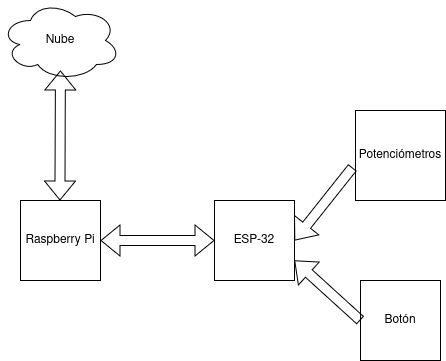
\includegraphics[width=1.1\textwidth]{DiagramaArquitectura.png}
\caption{Diagrama visual de la arquitectura a nivel de dispositivos del proyecto. Diagrama realizado con Draw.IO}
\end{figure}

\section{Diseño hardware}

Con respecto al diseño del Hardware, se ha decidido utilizar una arquitectura basada en microcontroladores, los cuales reciben información de aparatos electrónicos.

Se detalla más a fondo el hardware y los dispositivos electrónicos utilizados a lo largo del proyecto.

\subsection{Electrónica}

Se ha hecho uso de varios dispositivos electrónicos a lo largo del proyecto.

Muchos de estos dispositivos consisten en sensores de determinadas cantidades, por ejemplo; el botón mide si se ha pulsado este o no.

A continuación, se detallan los dispositivos electrónicos a los que se ha hecho uso a lo largo de este Trabajo de Fin de Grado; junto con una breve explicación de su funcionamiento

\subsubsection{Cables puente}

Los cables puente es un tipo de cableado con un conector en cada punta. Estos cables suelen ser utilizados en placas breadboard para conectar dispositivos electrónicos que se encuentren en columnas distintas del breadboard.\cite{eswiki:161708674}

\subsubsection{Placa de pruebas}

Una Placa de pruebas, o mejor conocido por el anglicismo \textit{breadboard}, es una placa electrónica que se utiliza para realizar circuitos electrónicos sin la necesidad de realizar soldaduras. Es generalmente utilizado en el desarrollo de prototipos, y contrasta con los circuitos soldados o circuitos impresos.\cite{eswiki:172543964}\cite{breadboard1}

\subsubsection{Botón pulsador electrónico}

Un button pulsador electrónico consiste en una resistencia que no deja pasar la corriente cuando se activa un pulsador.\cite{pushbuttonswitch}

\subsubsection{Potenciómetro}

Un potenciómetro consiste en una resistencia que se puede configurar con un mango. Un potenciómetro puede cambiar su resistencia con respecto al ángulo de rotación de forma linear o logarítmica.\cite{potentiometer1}

\subsubsection{Cableado USB (Universal Serial Bus)}

Se utiliza un cable USB en este proyecto para realizar comunicación entre el dispositivo Raspberry Pi 5 y el dispositivo ESP-32 (se explicarán estos en la siguiente sección). 

Este cable puede realizar funciones útiles en el desarrollo de sistemas empotrados; como cableado serial y de posibilidad de subir firmware a los microcontroladores. Es un cable muy versátil y de gran utilidad en el desarrollo de sistemas embebidos.

El cable específico que se utiliza para el proyecto es un cable USB-C a USB.

\subsection{Microcontroladores}

Los microcontroladores son dispositivos informáticos auto-contenidos que se utilizan para proporcionar funcionalidades informáticas variadas sin amplios gastos de electricidad.

En general, suelen ser utilizados cuando se precisa un control prácticamente completo del código que se ejecuta; han encontrado un nicho en el desarrollo de programas que comunican directamente con dispositivos electrónicos, o en el desarrollo de software con requisitos críticos de seguridad.

También se benefician de la limitada potencia eléctrica que se necesita para su funcionamiento, permitiendo a estos sistemas ejecutar programas durante años sin estar conectados a una fuente de electricidad constante.

\subsubsection{ESP-32 DevKit v4}

Este microcontrolador es una clase de microcontrolador desarrollado por la compañía EspressIf. \cite{espressif-1}

Dispone de las siguientes características relevantes a su funcionamiento. \cite{espressif-1} \cite{espressif-2}

\begin{enumerate}
 \item Un procesador ESP32-WROOM-32E
 \item Un chip puente UART-to-USB
 \item Un puerto USB-to-UART
 \item Un LED de 5V que se enciende cuando el dispositivo se enciende; es manipulable por los programas escritos a memoria FLASH
 \item Una serie de conectores, en forma de pines, que actúan como Entrada/Salida (pines ADC (Analog Digital Converter), RX, TX, GPIO, etc)
 \item Dos botones, uno de descarga, y otro de reinicio.
\end{enumerate}

\begin{figure}[H]
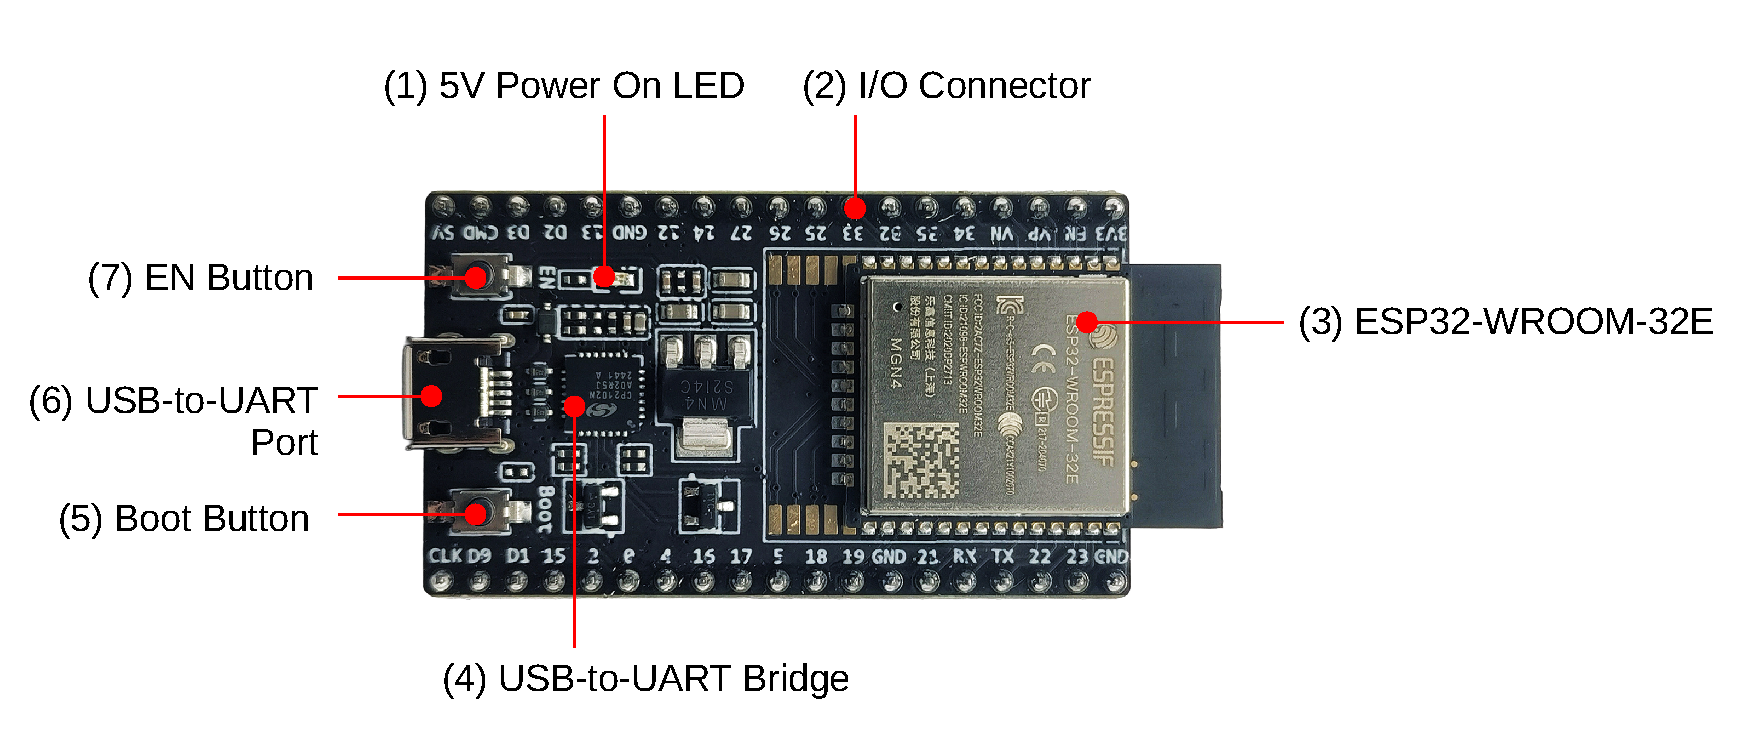
\includegraphics[width=1.1\textwidth]{esp32-devkitc-v4-functional-overview.png}
\caption{Listado de partes de microcontrolador ESP-32 DevKit v4~\cite{espressif-1}}
\end{figure}

Se incluyen múltiples y variadas funciones dentro del microcontrolador. Entre estas se incluye:

\begin{enumerate}
  \item \textbf{UEFI}: Es un protocolo de comunicaciones entre dispositivos utilizado de forma interna por el microcontrolador.
  \item \textbf{GPIO}: Es un tipo de pin que se utiliza como señal de entrada o de salida.
  \item \textbf{USB}: Es un protocolo de comunicación.
\end{enumerate}

\subsubsection{Alternativas consideradas}

Se consideró el dispositivo Arduino Uno para realizar el proyecto; al final no se utilizo debido a su precio más elevado, y por su más reducido rendimiento comparado con sus competidores.

También se consideró el dispositivo Raspberry Pico para realizar el proyecto como microcontrolador; pero se descartó debido a la falta de rendimiento comparado con el ESP-32.

\subsection{Diagrama de pines para el proyecto}

El dispositivo se conecta a tres dispositivos; utilizándose los siguientes pines:

\begin{enumerate}
 \item Un botón electrónico: Se conecta a los pines GPIO 13, a un pin de 5V, y a un pin de GND
 \item  Potenciómetro primero: Se conecta a los pines número 27, a un pin 3V3 y a un pin de GND
 \item Potenciómetro segundo: Se conecta a los pines número 33, a un pin 3V3 y a un pin de GND
\end{enumerate}

\begin{figure}[H]
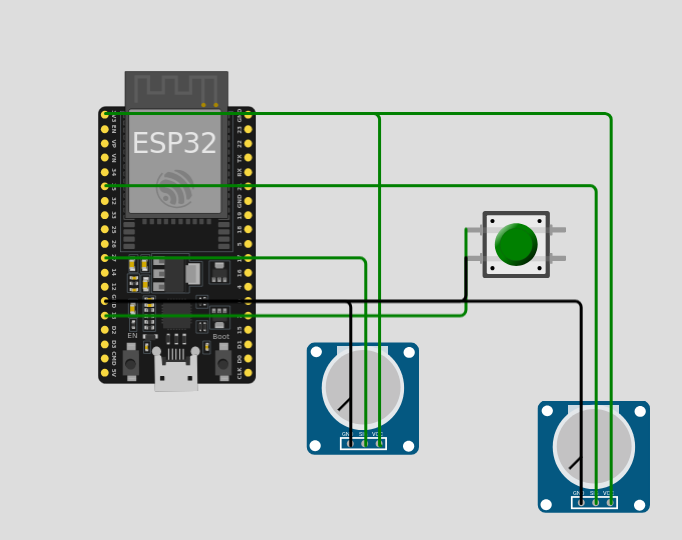
\includegraphics[width=1.1\textwidth]{espressdiagram.png}
\caption{Diagrama electrónico de conexiones del proyecto. Diagrama realizado con Wowki}
\end{figure}

\subsection{Ordenadores monoplaca}

\subsubsection{Introducción a los ordenadores monoplaca}

Los ordenadores, usualmente, se almacenan en una carcasa, suelen contener componentes tradicionalmente de gran envergadura, y no es trivialmente transportable.

Para solucionar este problema, se inventaron los ordenadores monoplaca, un ordenador completo que cabe dentro de una placa PCB (Printed Circuit Board)

\subsubsection{Raspberry Pi 5 16 GB}

El Raspberry Pi 5 es un ordenador monoplaca que viene en múltiples tipos; cada uno distinguido por la cantidad de memoria RAM de la placa.

\textbf{Características}

Las características principales de este dispositivo incluyen:

\begin{enumerate}
  \item Un procesador Broadcom BCM2712
  \item Una memoria RAM de 16GB
  \item Un puerto USB
  \item Un lector de tarjetas SD
\end{enumerate}

\subsubsection{Alternativas consideradas}

Existen varias versiones del Raspberry Pi 5 con menor capacidad de memoria RAM, estas al final no se escogieron para realizar este proyecto, aún siendo las recomendadas por el autor si se busca fabricar este producto de forma masiva por su menor coste, debido a que, al tratarse de un único prototipo no orientado a fabricarse de forma masiva por el momento, he decidido utilizar recursos más potentes al no conocer exactamente qué recursos harían falta para realizar este proyecto.

No se escogió tampoco Raspberry Pi 4 u otras versiones anteriores un el mismo motivo que las versiones más baratas del Raspberry Pi 5.

Tampoco se escogió un Mini-PC genérico. Este dispositivo es una compilación de hardware propia responsabilidad de su autor, lo cual dificultaría las tareas de aprendizaje inicial; la documentación de Raspberry OS y Raspberry Pi 5 me pareció mucho más completa para un proyecto del cual habían aún muchas incógnitas antes de su comienzo.

\section{Diseño software}
\subsection{Sistemas empotrados}

\subsubsection{Arquitectura software}

La arquitectura que se ha utilizado para el funcionamiento del software localizado en el sistema empotrado es una arquitectura \textbf{basada en módulos}.

Es una arquitectura principalmente basada en \textbf{polling}, para recibir y actuar con respecto a \textbf{eventos}, ya sea su proveniencia desde el cable USB-to-UART conectado al dispositivo, o de los dispositivos electrónicos a los que se encuentra conectado el microcontrolador a través de los cables puente.

No solo se reciben eventos; sino que la arquitectura también manda información a través del cable USB-to-UART para hacer conocer eventos que han ocurrido en el microcontrolador; por ejemplo, los valores de los dos potenciómetros, recogidos en tiempo real, a los que se encuentra conectado el microcontrolador.

\subsection{Software de sistemas}

\subsubsection{Arquitectura software}

La arquitectura que se ha utilizado para implementar este software dirigido a sistemas ha sido una \textbf{arquitectura modular}.

Esta arquitectura se distingue por la construcción de varios ejecutables, cada uno con funcionamiento independiente del otro, y ejecutables por separado. Todos los ejecutables, menos el que renderiza la interfaz gráfica de usuario, se comunican con una librería diseñada para poner en contacto cada evaluación con el microcontrolador; permitiendo a estos enviar a y recibir información de forma indirecta de los dispositivos electrónicos a través del microcontrolador.

Al igual que la arquitectura del software dirigido a los sistemas empotrados; esta también hace uso exhaustivo del \textbf{polling}, que escucha de forma reiterada unos \textbf{eventos}, los cuales suelen ser recibidos y procesados a partir de librerías y dispositivos externas; como lo puede ser la librería implementada en \textbf{serial.cpp}, que a su vez escucha eventos desde un dispositivo \textbf{USB-to-UART}; la librería externa \textbf{GTK} o la librería externa \textbf{SFML}

\subsection{Cliente local}

\subsubsection{Arquitectura software}

La arquitectura utilizada para el cliente local no es estrictamente la de un \textit{frontend} que se utilizaría en una arquitectura \textit{frontend-backend}. Esto se hace así principalmente por motivos de seguridad.

En una arquitectura típica \textit{frontend-backend}; el \textit{frontend} necesita de archivos informáticos para poder realizar funciones relativas al renderizado de componentes visuales; esto en general requiere desplegar un servidor web que albergue los ficheros del \textit{frontend}, y los pueda enviar en respuesta a peticiones específicas. Algunos servidores web comúnmente utilizados para esta tarea incluyen \textit{Apache Web Server} o \textit{Nginx}.

El problema es que en este tipo de aplicaciones, con requisitos muy estrictos de seguridad, queremos reducir a un mínimo los puertos a los que nuestro dispositivo, localizado en la clínica donde se realizan las evaluaciones, estará escuchando en todo momento con el objetivo de reducir lo más posible la superficie de ataque. Por eso este cliente se asemeja más a un cliente local que a lo que comúnmente se conoce como un \textit{frontend}.

Con respecto a la arquitectura software del cliente en si; su arquitectura software se basa fundamentalmente en el concepto del \textbf{entramado}; se le dan al usuario una amplia gama de posibles decisiones; y el programa se adapta a ellas e interpreta las decisiones por cada instrucción que se le indica al cliente.

\subsection{Cloud}

\subsubsection{Arquitectura software}

Se ha utilizado una arquitectura cliente-servidor para esta parte del trabajo.

Como busca desplegarse en máquinas que pueden tener características arbitrarias, y puede requerir de un traslado constante; se ha optado por utilizar una tecnología de despliegue para facilitar estos traslados denominada \textbf{Docker}.

Esta tecnología implementa el concepto de \textbf{contenedores}, donde en cualquier máquina en la que se pueda ejecutar el motor Docker, se creará un entorno informático apropiado para ejecutar el software.

El servidor utiliza \textbf{programación orientada a eventos} para recibir peticiones HTTPS por parte del cliente; y así comunicarse con una base de datos para realizar operaciones de lectura y de creación. No implementa un CRUD completo. Esta limitación de funcionalidad principalmente se ha realizado por motivos de seguridad; al haber menos eventos que puedan activarse en el sistema, es más reducida la posible superficie de ataque; algo fundamental en aplicaciones con requisitos estrictos de seguridad como lo puede un servidor desplegado al Internet abierto que almacena información sensible relativa a pacientes de un hospital/clínica.

Para desplegar y almacenar este contenedor; se ha optado por una máquina virtual, protegida por cortafuegos que solo autoriza conexiones de rangos de IP conocidos, realizada en el producto AWS EC2. (Amazon Elastic Computing Cloud)

\section{Arquitectura de datos}

\subsection{Gestor de bases de datos}

El gestor de bases de datos que se utiliza por defecto es denominado **MySQL**

\subsubsection{Configuración por defecto}

La configuración por defecto del gestor es la siguiente.

\textbf{Usuario}: root
\textbf{Contraseña}: root
No utiliza SSL por defecto

Se genera la siguiente información por defecto en la tabla \textit{profile}

Una fila con hospital\_username \textit{HOSPITAL\_MARIA\_CRISTINA} y hospital\_password un hash bcrypt2 iterado 10 veces de la contraseña \textit{GatitosLindos}

\subsection{Modelo de datos}

\subsubsection{Tabla \textit{profile}}

\textbf{\textit{hospital\_username}}

Aquí se almacena el nombre que utilizará el hospital para acceder a la tabla con sus datos asignados en la tabla \textit{test}

\textbf{\textit{hospital\_password}}

Aquí se almacena un hash de contraseña, junto con la semilla. Este es el formato que se utiliza: \textit{<hash bcrypt2>;<salt>}

\subsubsection{Tabla \textit{test}}

En esta tabla se incluyen todos los datos relativos a una evaluación completa por parte de un examinado en el contexto de una clínica u hospital examinador.

\textbf{\textit{id}}

En este campo se almacenan, de forma encriptada, los datos personales de los examinados.

Se almacenan los datos en el siguiente formato:

\textit{<texto cifrado>;<vector de inicializacion>}

\textbf{Formato de texto descifrado}

Consiste en el siguiente formato:

\textit{<Nombre y apellidos del examinado>\_<Número de identificación>\_<Frase generada al azar con un número indeterminado de caracteres>}

\textbf{\textit{first\_examination}}

En este campo se almacenan los resultados relativos a la primera evaluación de un examinado.

Se almacenan del siguiente modo:

\textit{<valor de t 1>,<valor de t 2>,<valor de t 3>}

\textbf{\textit{second\_examination\_*}}

En este campo se almacenan los resultados relativos a la segunda evaluación de un examinado.

Se almacenan del siguiente modo:

\textit{<valor de x para coche 1 o 2 en primer fotograma>,<valor de x para coche 1 o 2 en segundo fotograma>,<valor de x para coche 1 o 2 en tercer fotograma>}

\subsubsection{profile}

Esta base de datos incluye los datos relativos a hospitales; tiene dos campos, uno con el nombre del hospital, y otro con el hash de clave del hospital.

\subsubsection{tests}

Esta base de datos incluye un id, que consiste de datos personales encriptados de los examinados; y dos campos, uno para cada evaluación, que indica los movimientos realizados en cada evaluación.

%────────────────────── Chapter 3 — Implementación ────────────────────────────
\chapter{Implementación}

\section{Sistemas empotrados}

\subsection{Bucle principal}

El bucle principal se implementa dentro del fichero localizado en la raíz del proyecto, y denominado \textbf{main.c}.

Este bucle almacena tres mensajes, en codificación binaria \textit{UTF-8}, que indican acciones específicas a tomar al microcontrolador; principalmente, se indica a qué función relativa a la evaluación se debe llamar debido a que una evaluación va a comenzar de forma inminente en el sistema SBC, para inicializar la recepción de datos electrónicos relevantes a tal evaluación.

\subsection{Primera evaluación}

Esta parte se implementa dentro del fichero denominado first

Antes que nada, se comprueba que los pines GPIO hayan sido antes configurados como de entrada antes de comenzar el programa; de no ser así, devuelve un mensaje de error.

El resto del programa consiste en un bucle infinito que realiza las siguientes operaciones:

\begin{enumerate}
  \item Si se han configurado los pines GPIO, entonces el programa lee el voltaje digital; que interpreta como 0, o como 1.
  \item Si el programa lee que el voltaje obtenido no es 1 (es decir, el usuario ha accionado el botón y por tanto, no lee su propia corriente la placa), entonces, envía a través del cable serial un valor arbitrario, indicando que el botón se ha accionado.
  \item Por último, duerme 100 milisegundos antes de realizar un nuevo ciclo.
\end{enumerate}

\subsection{Segunda evaluación}

Esta parte se implementa dentro del fichero denominado second.c

Este programa sigue un bucle parecido al de la primera evaluación; pero con algunos cambios debido a la naturaleza analógica de los potenciómetros.

Antes que nada, se comprueba que los pines GPIO relevantes hayan sido antes configurados como de entrada antes de comenzar el programa; de no ser así, devuelve un mensaje de error.

El resto del programa consiste en un bucle infinito que realiza las siguientes operaciones:

\begin{enumerate}
  \item Si se han configurado los pines GPIO, entonces el programa lee el voltaje analógico; que interpreta como un voltaje específico.
  \item El programa configura los parámetros para el proceso ADC (Analog-to-Digital conversion)
  \item El programa lee y convierte el valor analógico en un valor digital utilizando los procesos ADC anteriormente configurados
  \item Por último, duerme 10 milisegundos antes de realizar un nuevo ciclo.
\end{enumerate}

\subsection{Utilidades relativas a dispositivos UART}

Esta parte se implementa dentro del fichero denominado \textit{uart.c}

Antes que nada, se comprueba que el dispositivo UART relevante haya sido antes configurado antes de comenzar el programa; de no ser así, devuelve un mensaje de error.

\begin{enumerate}
\item Primero, se configura el dispositivo UART; por defecto, no se asume un dispositivo UART externo; sino un dispositivo UART interno UART-to-USB
\item Después, cada vez que se llame a read\_from\_uart, se realiza una lectura según la configuración; y se devuleve un valor según el valor que haya obtenido por el dispositivo UART, dependiendo del mensaje enviado 
\end{enumerate}

\section{Software de sistemas}

\subsection{Primera evaluación}

Aquí se implementa todo lo relativo a la primera evaluación, la prueba de tiempo de anticipación.

Más o menos, el funcionamiento consiste en lo siguiente:
\begin{itemize}
  \item Primero se inicializan los parámetros, clases y valores relativos a la evaluación.
  \item Después se entra en un bucle, donde se comprueba si se ha mandado información por el dispositivo serial, y si es así, reinicia la evaluación o termina la evaluación.
  \item Al finalizar la evaluación, guarda toda la información recolectada sobre este para su auditoría, y cierra el programa de forma automática
\end{itemize}

\begin{figure}[H]
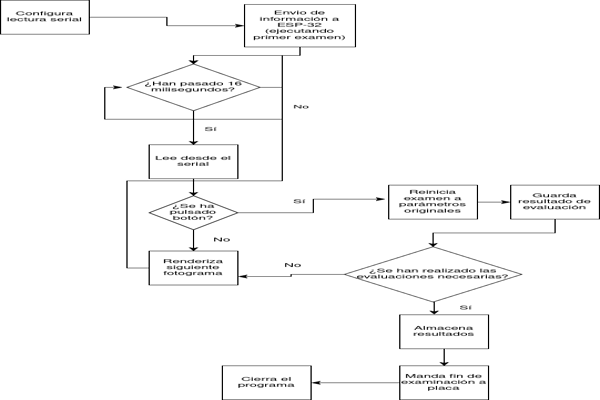
\includegraphics[width=1.1\textwidth]{DiagramaPrimeraEvaluacion_resized.png}
\caption{Diagrama visual del flujo de ejecución de la primera evaluación. Diagrama realizado con Draw.IO}
\end{figure}


\subsection{Segunda evaluación}

Aquí se implementa todo lo relativo a la primera evaluación, la prueba de coordinación mano-ojo.

Tiene un funcionamiento algo más complejo que la otra evaluación.

\begin{itemize}
  \item Primero se inicializan todos los parámetros, clases y valores; incluidos una serie de vallas, posiciones, y dos lookup tables; uno asociado con cada potenciómetro.
  \item Se calculan una serie de parámetros para inicializar de forma correcta los lookup tables
  \item Después, se entra en un bucle; donde se obtiene el voltaje recibido del potenciómetro respectivo, y se realizan los siguientes pasos:
  \subitem Se obtiene el lookup table que corresponde al potenciómetro del que proviene el voltaje
  \subitem Se transforma este voltaje a un índice en el lookup table.
  \subitem A partir de este índice calculado, obtenemos una posición de x
  \subitem El vehículo asociado al potenciómetro donde viene el voltaje se desplaza hacia al valor en x obtenido.
  \subitem Terminado esto, indica que el siguiente valor de voltaje recibido corresponderá al otro potenciómetro.
  \item Por último, si no se han terminado aún las posiciones que podemos asignar a las vallas, se asignan las siguientes posiciones.
  \item Si hubiesen terminado las posiciones que podemos asignar, se guarda toda la información recolectada sobre la evaluación para su auditoría, y cierra el programa de forma automática
\end{itemize}
    
\begin{figure}[H]
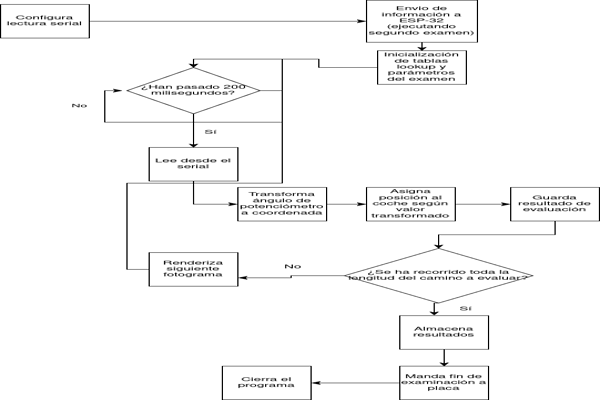
\includegraphics[width=1.1\textwidth]{DiagramaSegundaEvaluacion_resized.png}
\caption{Diagrama visual del flujo de ejecución de la segunda evaluación. Diagrama realizado con Draw.IO}
\end{figure}

\subsection{Utilidades UART}

Este programa se encarga de proporcionar configuraciones, y métodos para configurar un dispositivo serial, leer de este, y mandar información a través de este; asume que el dispositivo del que lee y escribe ejecuta el sistema software es el descrito en la sección de diseño.

Antes que nada, se comprueba que el dispositivo UART relevante haya sido antes configurado antes de comenzar el programa; de no ser así, devuelve un mensaje de error.

\begin{enumerate}
\item Primero, se configura el dispositivo UART; por defecto, no se asume un dispositivo UART externo; sino un dispositivo UART interno UART-to-USB
\item Después, cada vez que se llame a read\_from\_uart, se realiza una lectura según la configuración; y se devuleve un valor según el valor que haya obtenido por el dispositivo UART.
\end{enumerate}

\section{Cliente local}

\subsection{Recolección de datos de evaluación}

Hay una opción en el programa que permite recolectar los datos de un examinado; este es el flujo de funcionamiento:

\begin{enumerate}
  \item Se intenta acceder a tres archivos:
  \item[\textbullet] first\_examination.txt: Con los datos de evaluación del primer examen
  \item[\textbullet] second\_examination.txt: Con los datos de evaluación del segundo examen
  \item[\textbullet] hospital\_credentials.txt: Con los datos de identificación para el hospital.
  \item Si se localizan estos archivos, se empieza preguntando nombre y apellidos del usuario.
  \item Después, se pide tipo de documento; puede ser un DNI español, o un número NIE 
  \item Se pide el número de documentación escogido, más la letra; se contrasta que el número proporcionado corresponde con la letra proporcionada; si no es así, el número se considera inválido y se lanza un mensaje de error.
  \item Se muestra un formulario para confirmar los datos.
  \item Se encriptan los datos personales del usuario con unos parámetros de encripción cargados o generados en segundo plano al iniciarse la aplicación; y se envían los datos de evaluación al servidor.
\end{enumerate}


\subsection{Recepción de información}

Esta opción permite obtener los datos de evaluación de todos los usuarios examinados dentro del dispositivo; su flujo de funcionamiento es el siguiente:

\begin{enumerate}
  \item Se intenta acceder a hospital\_credentials.txt, un archivo con datos de identificación para el dispositivo asociado a un hospital.
  \item Se envía una petición al servidor en nube para que reciba los datos y los envíe al cliente.
  \item El cliente genera un archivo HTML, que consiste de una tabla simple donde se muestra toda la información asociada al hospital; y desencriptada por completo.
  \item Se escribe el archivo y se cierra el programa.
\end{enumerate}

\subsection{Utilidades de encriptación y desencriptación de datos}

Para encriptar los datos se utiliza una clave AES-256; para obtener esta clave, se sigue el siguiente flujo:

\begin{enumerate}
  \item Se intenta localizar el archivo denominado encryptionparameters.txt; si este existe, se carga la clave ya existente de ahí como buffer binario.
  \item En caso de no existir, se genera una clave al azar. Esta clave se guarda en formato hexadecimal en el archivo encryptionparameters.txt
\end{enumerate}

Para la encriptación y desencriptación de los datos; el proceso es muy parecido entre sí; se introduce el texto a encriptar/desencriptar, se pasa ese texto por un cifrador/descifrador, y se devuelve el texto encriptado/desencriptado.

\subsection{Utilidades para comunicación con interfaces cloud}

Se utiliza como utilidad principal la librería \textbf{Axios}.

Este es el flujo con el que se mandan peticiones al servidor:

\begin{enumerate}
  \item Se recibe un objeto JSON, que contiene todos los parámetros relevantes para el \textit{endpoint} que se busca llamar en el servidor en nube.
  \item Se inicializan todos los campos HTTP relevantes a cada petición, esto incluye el método HTTP (GET o POST), y la dirección URI a la que se busca enviar la petición.
  \item Se devuelve una promesa, un tipo de datos asíncrono, que permite devolver una instancia de un tipo concreto sin bloquear el programa en espera de este.
\end{enumerate}

\subsection{Utilidad para introducción y validación de datos de documentación española}

\begin{enumerate}
\item Primero, se pide al usuario que otorgue su tipo de documento (Documento Nacional de Identidad o Número de Identidad de Extranjero)
\item El programa recoge el número correspondiente
\item Se verifica que la letra introducida sea la correcta según las reglas de la normativa oficial Española para el cálculo de dígitos de control. \cite{digitocontrol}
\item Si no se verifica correctamente; se pedirá al usuario que vuelva a introducir su número, y la letra esperada para el número que introducieron.
\end{enumerate}

\section{Servidor en nube}

\subsection{Contenedor de bases de datos}

Este contenedor utiliza el gestor de bases de datos MySQL, y por defecto instala su última versión disponible en el Docker Hub.

Por defecto, se inicializa un usuario root con clave root; y se inicia un esquema con un hospital de ejemplo; con los siguientes parámetros con carácter demostrativo:

\begin{itemize}
 \item Usuario: HOSPITAL\_MARIA\_CRISTINA
 \item Clave: GatitoPerez
\end{itemize}

\subsection{Contenedor de servidor cloud}

Este es un contenedor que por defecto instala NPM, las dependencias del proyecto; e inicializa un servidor que escucha en localhost:3000 por defecto.

Está pensado para que un servidor externo web haga proxy con este servidor; pero si se quiere que el servidor escuche a cualquier dirección IP (o dominio) que le llegue de forma directa, sin proxies, se debería cambiar localhost por 0.0.0.0, o a la IP que se quiera escuchar.

Dispone de varios componentes lógicos:

\subsubsection{API REST}

El API REST implementa un CRUD parcial con funciones de lectura de todos los datos relativos a un hospital en concreto, dado un nombre de hospital y una clave; y una función para agregar una nueva fila a la base de datos.

El flujo general de datos consiste en el siguiente:

\begin{enumerate}
  \item Primero, se obtiene el nombre del hospital en la petición. Si el hospital no existe; se devuelve un mensaje de clave incorrecta para esconder la verdadera causa del error, por motivos de seguridad.
  \item Después, se obtiene la clave del hospital; esta se compara con el hash bcrypt2 existente en la base de datos asociada al nombre del hospital; si coincide esta clave con el hash, se procede al siguiente paso.
  \item Se realiza la acción pedida, ya sea crear una nueva fila de datos en la base de datos; o devolver, para el hospital elegido, toda la tabla completa.
\end{enumerate}

No se ofrecen opciones más específicas para devolver datos individuales o de filtrado de datos en remoto, ya que prácticamente toda la información en la base de datos remota se asume encriptada; y no legible por el servidor remoto

\subsubsection{Utilidades}

Se incluyen funcionalidades para realizar comparación de contraseñas recibidas con hashes en base de datos.

Las contraseñas se asumen en hash bcrypt2, con 10 iteraciones por defecto.

%────────────────────── Chapter 4 — Funcionamiento ────────────────────────────
\chapter{Funcionamiento}

\section{Flujo de usuario}

Dividiremos a los posibles tipos de usuarios en cuatro posibles tipos:

\subsection{Examinado}

Primero, el examinado llega a la sala. A este se le explicará el procedimiento para la primera evaluación; la realizará.

Después, el examinado le es explicado la segunda evaluación; la realiza.

Por último, el examinado ofrece sus datos; documento identificativo y su número; además de su nombre y apellidos.
\subsection{Doctor}

El doctor recibe al examinado; abre el programa de evaluación; abre el primer programa de evaluación y espera a que el examinado termine; entonces abre el siguiente.

El doctor abre el programa para recolectar los datos del examinado; pulsa 2 para comenzar el proceso de envío; cuando el programa lo indica, invita al examinado a leer y firmar la política de protección de datos; tras firmar manda los datos al servidor.

Al pedirlo un auditor; el doctor proporcionará los datos de evaluación encriptados para corregirlos; y bajo orden judicial, proporcionará los datos del examinado asociados a una evaluación; mandando los datos relevantes desencriptados.

\subsection{Auditor}

El auditor pide acceso a los datos encriptados de cada hospital para auditar las evaluaciones y que se hayan puntuado correctamente.

Puede, por orden judicial; recibir datos desencriptados relativos a la situación judicial immediata

\subsection{Atacante}

El atacante intenta acceder a la base de datos de hospitales escaneando las IPs del mundo; no encuentra nada ya que no está en la red correcta.

No dándose por vencido; entra en un hospital y consigue acceder a la red y al endpoint. El atacante descubre que carece de una clave de hospital; por lo que el sistema no le deja acceder a datos.

El atacante consigue acceder a la máquina cloud y roba la base de datos del hospital; al estar los datos encriptados, no sabe de quién son cada examen.

El atacante intenta encontrar información comparando hashes; al incluirse con los datos personales cada examinado un string aleatorio; los hashes son completamente distintos los unos de los otros incluso para los mismos datos personales; el atacante no saca nada en claro.

El atacante entra en una habitación, accede al dispositivo del doctor, consigue desencriptar los datos de todo el hospital en un descuido; y confiado intenta acceder a los datos de otro hospital; no puede, ya que cada clave de hospital es única y generada al azar; y solo ha conseguido atacar a ese hospital en concreto; el resto sigue seguro

\section{Demo en formato vídeo}

Se ofrece dentro del repositorio una serie de vídeos demostrativos.

Se demuestra la funcionalidad de evaluación a partir de la realización de las dos evaluaciones, utilizado los dispositivos electrónicos a tal efecto; y también se ofrece una demostración de adición de un examinado y sus resultados al servidor en nube, junto con su posterior recepción como archivo .html

\chapter{Pruebas}

\section{Sistemas empotrados}

Se han realizado algunas pruebas en el software dirigido a sistemas empotrados; sobre todo se prueban métodos que implementan la utilidad que permite leer y escribir de dispositvos UART. Estos tests se realizan bajo la suite de tests Unity.

\subsection{Instrucciones de compilación}

\begin{enumerate}
  \item Instale ESP-IDF
  \item Inicialize ESP-IDF con el comando \begin{verbatim}source "\$HOME/.espressif/tools/activate\_idf\_<version>.sh"\end{verbatim} 
  \item Acceda al directorio test
  \item Realize la configuración que desee con \begin{verbatim}idf.py menuconfig\end{verbatim}
  \item Ejecute el comando \begin{verbatim}idf.py -p <port> build\end{verbatim}
\end{enumerate}

\subsection{Métodos probados y resultados}

Con respecto a pruebas; se prueban dos casos:

\begin{enumerate}
  \item ¿Puedo inicializar un programa de evaluación sin antes configurar el entorno?
  \item ¿Se lee desde el dispositivo UART bien una información que sé me va a llegar?
\end{enumerate}

\section{Software de sistemas}

Se han realizado algunas pruebas en el software de sistemas; se prueban los métodos dentro de cada fichero implementado de evaluación, asumiendo unos parámetros definidos específicos. Estos tests se realizan bajo la suite de tests GoogleTest.

\subsection{Instrucciones de compilación}
  
  \begin{enumerate}
  \item Descargar e instalar CMake
  \item Acceder al directorio raíz del proyecto.
  \item Modifique dentro del archivo \begin{verbatim}CMakeLists.txt\end{verbatim} la opción TEST a True
  \item Ejecutar el comando \begin{verbatim}cmake .\end{verbatim} Esto sirve para generar los archivos .make correctos 
  \item Ejecutar el comando \begin{verbatim}cmake --build .\end{verbatim} Los binarios se guardarán en la carpeta bin/
  \end{enumerate}

\subsection{Métodos probados y resultados}

\subsubsection{Común a ambas evaluaciones}

\begin{enumerate}
 \item \textbf{InitShapeInitsShapeWithCorrectPosXAndPosY}: Se prueba que el método initShape con los parámetros $x=35$ e $y=35$ resultará en una instancia de sf::RectangleShape siendo generada con posición en x igual a 35, e posición en y igual a 35.
 \item \textbf{InitShapeInitsShapeWithCorrectPosXAndPosYAndSize}: Se prueba que el método initShape con los parámetros $x=35$, $y=35$, $sizeX = 45.0f$ e $sizeY = 45.0f$ resultará en una instancia de sf::RectangleShape siendo generada con posición en x igual a 35, posición en y igual a 35, tamaño x igual a 45.0f e tamaño y igual a 45.0f.
 \item \textbf{InitCarActuallyInitsTheCar}: Se prueba que el método initCar con los parámetros $x=200$ e $y=200$ resultará en una instancia de sf::RectangleShape siendo generada con posición en x igual a 200, posición en y igual a 200; y posición "real" para coordenada igual a la posición en x para cada coordenada.
\end{enumerate}

Todas estas pruebas resuelven correctamente en la versión última del respositorio remoto.

\subsubsection{Específicos a primera evaluación}

\begin{enumerate}
  \item \textbf{ResetTestActuallyAffectsTheCar}: Se comprueba que el método pensado para reiniciar la evaluación a sus parámetros determinados efectivamente realiza esta acción
\end{enumerate}

Todas estas pruebas resuelven correctamente en la versión última del respositorio remoto.

\subsubsection{Específicos a segunda evaluación}

\begin{enumerate}
\item \textbf{InitializeWallsInitializesWallsCorectly}: Se prueba que el método initializeWalls, dada un array vacio de instancias sf::RectangleShape con tamaño NUMBER\_OF\_WALLS; un tamaño de "pared" en las coordenadas x e y, y una posición inicial de la primera "pared" devolverá un array de paredes con la posición indicada en x; y los tamaños indicados para x e y en cada pared
\item \textbf{InitializePositionsInitializesPositionsCorectly}: Se prueba que el método initializePositions, dado un array vacio de valores primitivos enteros (int), devolverá un array con todas las posiciones teniendo un valor de 10, 0 o -10
\item \textbf{InitializeLookUpTableInitializesTableCorectly}: Se prueba que el método initializeLookUpTable, dado un radio del rango de valores máximo y mínimo de un potenciómetro con la longitud de la pantalla en x; y una colección igual al rango de posiciones del potenciómetro multiplicada por el radio anteriormente redondeado a entero por lo bajo; devolverá un array de enteros donde solo cambiará el valor asignado cada vez que se cuente un número "radio" de elementos dentro de ese array
\item \textbf{PositionsAreAssignedCorrectly}: Se comprueba que para un array de posiciones y un array de "paredes", las posiciones se asignan correctamente.
\item \textbf{VerifyCollisionVerifiesCorrectly}: Se comprueba que la función verifyCollision resuelve colisiones correctamente según la función matemática de colisión descrita en el apartado 2.2.1 de esta memoria
\item \textbf{VerifyResolvePosition}: Se comprueba que se resuelven colisiones correctamente para casos en los que el valor voltaje simulado se encuentra dentro del rango esperado del potenciómetro; y en casos en los que da un valor no dentro del rango esperado del potenciómetro (ya sea menor o mayor al valor asumido dentro del rango)
\end{enumerate}

Todas estas pruebas resuelven correctamente en la versión última del respositorio remoto.

\section{Cliente local}

Se han realizado algunas pruebas en el cliente local; sobre todo sobre las funciones relativas a las utilidades. Estos tests se realizan bajo la suite de tests Jest.

\subsection{Instrucciones de compilación}

\begin{enumerate}
  \item Descarga e instala Node
  \item Ejecuta el comando \begin{verbatim}npm install\end{verbatim}
  \item Ejecuta el comando \begin{verbatim}npm test\end{verbatim}
\end{enumerate}

\subsection{Métodos probados y resultados}

Con respecto a pruebas; se prueban dos casos:

\begin{enumerate}
  \item ¿A partir de un número de documentación, este lo valida correctamente según la normativa española?
\end{enumerate}

\section{Servidor en nube}

Se han realizado algunas pruebas en el servidor en nube; sobre todo sobre las funciones relativas a las utilidades. Estos tests se realizan bajo la suite de tests Jest.

\subsection{Instrucciones de compilación}

\begin{enumerate}
  \item Descarga e instala Node
  \item Ejecuta el comando \begin{verbatim}npm install\end{verbatim}
  \item Ejecuta el comando \begin{verbatim}npm test\end{verbatim}
\end{enumerate}

\subsection{Métodos probados y resultados}

%────────────────────── Chapter 5 — Discusión ─────────────────────────
\chapter{Conclusiones}

En esta memoria se ha desarrollado por escrito, y se ha explicado, una suite de evaluaciones psicotécnicas para conductores.

Como se ha podido ver, se trata de un prototipo y una prueba de concepto, de lo que podrían ser las bases de un sistema de evaluación psicotécnica para conductores mucho más complejo y desarrollado, incluso parte de un futuro dispositivo médico en el futuro.

Aún siendo un prototipo, se han implementado componentes para prácticamente todas las funcionalidades básicas que se podría esperar de este tipo de sistemas; utilizando buenas prácticas como la documentación, las pruebas, el cuidado en el rendimiento, y la multidisciplinaridad.

\section{Limitaciones y posibles mejoras}

El autor se hace cargo de las limitaciones de esta suite software para la puesta en práctica immediata; ya que no se ha consultado directamente con expertos en los campos trabajados, como lo pueden ser psicólogos especialistas en cognición, médicos, y otros perfiles relevantes dentro de la industria y la academia; este trabajo está pensado como base tecnológica y como demostración de una posible recreación con tecnologías modernas, todo publicado bajo licencias permisivas, para un posible dispositivo médico futuro. No está pensado para de por sí poder utilizarse directamente en el proceso de evaluación médica de pacientes.

La interfaz de usuario puede no ser muy apropiada para perfiles de usuario típicos; aunque se ha intentado mitigar esto realizando scripts de instalación y de ejecución que simplifican este proceso, haciendo examinaciones muy visualmente contrastadas en términos de colores, y realizando vídeos demostrativos, manuales de instalación y de usuario; se requiere de un proceso instalación manual de dependencias externas y la configuración de un entorno electrónico apropiado para el funcionamiento correcto del sistema completo.

Este proyecto no es portable a otros entornos informáticos; asume un entorno hardware y software muy específico en los parámetros configurados por defecto; y cualquier desviación puede resultar en el no correcto funcionamiento de componentes de la suite software. 

Debido al precio que exige tener una instancia en nube encendida durante semanas o incluso meses, por el uso de AWS como tecnología en nube escogida, y por las políticas de precio por uso que existen en proveedores IaaS de forma general; y además, debido a que la configuración con HTTPS requiere de una dirección IP constante para la máquina, y un dominio web que asignar a esta dirección IP, se utiliza una conexión desencriptada con el servidor; al probar una configuración HTTPS en nube, debido a estas restricciones principalmente financieras, había de forzar a mi cliente local a confiar en cualquier certificado que le llegase; lo cual impidió una configuración completa de flujo HTTPS.

%────────────────────── Appendices ─────────────────────────────────────
\begin{umaappendices}

\umaappendix{Manual de usuario}

En este manual de usuario se busca introducir a todos los tipos de usuario, de forma sencilla, y paso por paso, a un uso adecuado de esta suite de software.
\section{Para el usuario}

\subsection{¿Cómo realizar una evaluación?}

Para las evaluaciones, lo más importante es la pantalla, y los botones o manivelas que hayas de utilizar. Cuando actuas sobre los botones o las manivelas, esto causará efectos en la pantalla, que están hechos para que se puedan visualizar fácilmente.

Tu doctor te hará dos tipos de evaluación, vamos a entrar un poco más en detalle en los exámenes que habrás de realizar:

\subsubsection{Primera evaluación}

La primera evaluación busca medir tu tiempo de anticipación. Vamos a mostrar una fotografía de lo que probablemente vas a ver en la pantalla:

\begin{figure}[H]

\includegraphics[width=1.1\textwidth]{pantalla1.png}
\caption{Ejemplo visual de la primera evaluación}
\end{figure}

Tu objetivo en esta evaluación consiste en, cuando el coche, representado por el cuadradito blanco, entre en el tunel, representado por el cuadrado grande por la izquierda; debes intentar anticiparte, y pulsar el botón cuando creas que el coche va a salir por la derecha.

El examen se repite tres veces; y en cada una, deberás hacer lo mismo; el programa se cerrará cuando haya concluido el examen.

\subsubsection{Segunda evaluación}

La segunda evaluación busca medir tu coordinación mano-ojo, utilizarás las dos manivelas que podrás ver en la pantalla. Aquí mostramos una foto de lo que verás durante el examen:

\begin{figure}[H]

\includegraphics[width=1.1\textwidth]{pantalla2.png}
\caption{Ejemplo visual de la segunda evaluación}
\end{figure}

Tu objetivo en esta evaluación consiste en mantener los coches, representados por los cuadraditos blancos, dentro de cada carretera; hay una carretera por cada coche. Esta carretera tiene curvas, y tu objetivo será mantener los dos cuadraditos en todo momento dentro de su carretera. El cuadradito de la izquierda tendrá que circular en la carretera de la izquierda en todo momento, y el cuadradito de la derecha tendrá que circular en la carretera de la derecha en todo momento.

Cuando haya terminado el examen, el programa se cerrará.

\subsection{¿Cómo subo una evaluación?}

Tu doctor abrirá un programa donde tendrás que introducir los siguientes datos:

\begin{enumerate}
  \item Un nombre y apellidos personales.
  \item Un tipo de documento de identificación (puede ser un documento DNI o NIE) 
  \item Un número de documento de identificación
\end{enumerate}

Tu doctor te proporcionará un formulario físico, aquí se incluyen los derechos que tienes relativos a tus datos personales, y qué se va a hacer con ellos; leelo con atención, plantea todas las dudas que tengas, y si consientes al tratamiento indicado, firma el documento.

Después, se mostrará en la pantalla si quieres confirmar que todos tus datos se vayan a subir a la nube. Lee bien y comprueba que los datos en pantalla es lo que de verdad quieres subir; cuando hayas concluido esto, tus datos ya estarán subidos.

\section{Para el doctor}

\subsection{¿Qué evaluaciones se utilizan?}

\subsubsection{Primera evaluación}

La primera evaluación que se realiza se trata del test del tunel, originalmente basado del estudio por MARUYAMA, KINYA y KITAMURA, SEIRO en 1966 \cite{maruyama1966speed}

\subsubsection{Segunda evaluación}

La segunda evaluación que se realiza se trata del test del laberinto, originalmente derivado del polireactografo explicado en el libro por Bonnardel, Raymond en 1943 \cite{bonnardel1943adaptation}

\subsection{¿Cómo cargo los programas de evaluación?}

Los programas de evaluación han de accederse a través de la carpeta \textit{bin/} que se pueden encontrar en la carpeta \textit{SystemSoftware/Integrated}. Hay dos programas, estos son:

\textit{gui}: Una interfaz sencilla que permite abrir los dos programas de evaluación sin tener que acordarte de dónde está cada programa.

\textit{first\_examination}: Este programa es la primera evaluación

\textit{second\_examination}: Este programa es la segunda evaluación

Has de abrir los programas para cada examen, y dar instrucciones al examinado sobre cómo realizar cada examen; preferiblemente deberías realizar una demostración, para luego que puedan hacer el examen real.

\subsubsection{Interpretación de los datos}

Los datos se cargan en dos archivos de texto; estos se denominan:

\textit{first\_examination.txt}: Mide el tiempo de pulsación; no pasa nada si no corresponde a los segundos exactos que el examinado tardó en pulsar. El valor óptimo debería ser alrededor de 0.90.

\textit{second\_examination.txt}: Mide la posición de los dos coches a lo largo del examen.

\subsection{¿Cómo subo los datos del usuario?}

Debes copiar en el directorio \textit{Web/Integrated/build} los archivos \textit{first\_examination.txt} y \textit{second\_examination.txt}. Tras hacer esto, deberás correr el siguiente comando en la terminal: \textit{npm run dev}.

Se mostrará una pantalla donde puedes escoger entre varias opciones, la que interesa para subir los datos será la opción número 1.

Antes de pulsar la opción, presenta al usuario con un formulario de política de protección de datos. \textbf{Asegurate que el usuario firma este formulario antes de subir la información}.

A partir de aquí, después de que el usuario introduzca sus datos, antes de subirlo deberías dar tiempo al usuario para que lea y comprenda todo bien y que todo sea correcto.

Se incluye un ejemplo de caso de uso de introducción de los datos:

\begin{verbatim}
¡Bienvenido/a!
*****************************************
OPCIONES:
1. Agregar una examinacion al sistema
2. Obtener todos las examinaciones del hospital
3. Salir del programa
1

Files have been found correctly.
Nombre del examinado: Pepe Perico Perez

Tipo de documento en uso (DNI/NIE): AAA
Error, tipo de documento invalido

Tipo de documento en uso (DNI/NIE): DNI
DNI del examinado (con letra incluida): 48902777E

Letra del DNI incorrecta. Compruebe el numero de DNI escrito
Letra de DNI esperada: Q
Letra de DNI obtenida: E
Error, numero de documento incorrecto; vuelva a indicarlo, por favor

DNI del examinado (con letra incluida): 48902777Q
Nombre introducido: Pepe Perico Perez
Tipo de documento: DNI
Numero de documento: 48902777Q
¿Proceder a la subida? (s/n) n

Vuelva a introducir sus datos de nuevo
Nombre del examinado: Pepe Perico Perez
Tipo de documento en uso (DNI/NIE): NIE
DNI del examinado (con letra incluida): X8947338R

Letra del NIE incorrecta. Compruebe el numero de NIE escrito
Letra de NIE esperada: Q
Letra de NIE obtenida: R
Error, numero de documento incorrecto; vuelva a indicarlo, por favor

DNI del examinado (con letra incluida): X8947338Q
Nombre introducido: Pepe Perico Perez
Tipo de documento: NIE
Numero de documento: X8947338Q
¿Proceder a la subida? (s/n) s
\end{verbatim}

\subsection{¿Cómo puedo obtener todos los datos de cada usuario?}

Deberás abrír el directorio \textit{Web/Integrated/build}, y correr el siguiente comando en terminal \textit{npm run dev}.

Si no habías ejecutado el programa nunca jamás hasta ahora, debes comprobar primero si existe un archivo denominado \textit{encryptionparameters.txt}, si ese archivo existiese sin haber nunca abierto este programa, \textbf{debe descartarse el dispositivo immediatamente y pedir la instalación de un dispositivo nuevo, con credenciales actualizadas}.

Se mostrará una pantalla donde puedes escoger entre varias opciones, la que interesa para subir los datos será la opción número 2. Se generará automáticamente un archivo llamado \textit{html\_results.html}; donde se incluirán los datos de los examinados en forma de tabla.

Se muestra aquí un ejemplo de un posible fichero \textit{html\_results.html}

\begin{verbatim}
<html>
  <head></head>
  <body>
    <table>
      <tbody>
        <tr>
          <th>Datos de paciente</th>
          <th>Resultados primer examen</th>
          <th>Resultados segundo examen 1</th>
          <th>Resultados segundo examen 2</th>
          </tr>
        <tr>
          <td>PEPE PERICO PEREZ_X947338Q_MLovpPMAbuUriGChJ4kY</td>
          <td>0.025000,1.559999,0.814999</td>
          <td>2,2,2,2,2,2,2,2,2,2,2,2,2,2,2,2,2,2,2,2,2,2,2,2,2,2,2,2,2,42,74,80,80,80,79,79,78,77,80,79,79,81,106,129,140,146,153,158,158,151,135,131,131,140,143,145,144,144,147,166,174,176,170,154,143,141,138,131,127,124,123,126,132,134,135,138,140,142,129,116,98,93,92,92,78,57,35,26,22,24,23,22,24,23,23,24,23,23,23,23,24,24,23,11,2,2,2,2,2,13,28,31,31,33,42,42,42,43,42,42,42,42,44,42,42,42,42,42,42,42,42,42,44,45,39,40,40,40,41,42,42,42,43,42,42,43,42,42,42,42,42,45,57,65,55,32,15,2,2,2,5,32,52,73,87,92,98,98,98,99,98,98,95,67,31,26,39,44,51,53,54,57,67,65,68,68,71,69,63,53,46,48,56,62,72</td>
          <td>599,599,599,599,599,599,599,599,599,599,599,599,599,599,599,599,599,599,599,599,599,599,599,599,599,599,599,599,599,599,599,599,599,599,599,599,580,556,536,516,499,499,499,497,472,444,426,418,418,422,443,447,449,437,422,419,419,419,418,415,387,379,379,385,389,393,398,403,413,424,426,425,419,409,393,382,370,368,374,387,397,405,406,406,406,408,424,432,436,435,429,413,384,354,336,335,336,334,342,373,392,395,394,396,396,395,395,396,394,394,395,396,396,395,395,395,394,387,360,354,387,420,446,469,497,500,502,501,506,506,507,506,506,507,507,506,506,506,507,509,509,510,509,510,510,510,510,510,510,510,510,509,510,509,510,510,509,499,491,488,489,490,490,493,498,511,524,524,504,478,459,450,447,447,447,447,455,471,483,497,503,504,505,511,512,518,518,517,515,508,500,498,506,521,529</td>
        </tr>
      </tbody>
    </table>
  </body>
</html>
\end{verbatim}

\section{Para el auditor}

\subsection{¿Cómo puedo realizar auditoría de los datos?}

Podrás obtener acceso a partir de las credenciales de cada hospital a los datos que se contienen en ellos; a partir de ahí, podrás obtener una tabla con todas las evaluaciones realizadas.

Todos los datos escritos relativos a las pruebas se deben verificar con la misma versión del programa con la que se han generado, de no ser así, se puede llegar a conclusiones erróneas.

\subsection{¿Qué datos tengo disponibles para auditar?}

Tendrás datos de los examinados respecto a sus acciones en los exámenes de tiempo de anticipación y de coordinación mano-ojo.

Para el primer examen, se mide el tiempo de pulsación; no pasa nada si no corresponde a los segundos exactos que el examinado tardó en pulsar. El valor óptimo debería ser alrededor de 0.90.

Para el segundo examen, se mide la posición de los dos coches a lo largo del examen.

\subsection{He encontrado un usuario que no debería haber aprobado por motivos médicos, ¿qué puedo hacer?}

Puedes, por orden judicial, pedir que se desencripten los datos asociados al usuario, y que se verifique si esta persona se le ha autorizado el tener el carnet de conducir, o no.

Por defecto todos los datos personales de usuarios se encuentran encriptados, por lo que no podrás acceder a ellos hasta que una orden judicial exija su desencriptación.

\umaappendix{Manual de instalación}

\section{Instalación general del proyecto}

Existe un archivo install.sh en la raiz del proyecto, y otro run.sh; ejecuta esos archivos y debería realizarse todo con éxito

\section{Instalación de hardware}

\section{Instalación de software para sistemas empotrados}

\begin{enumerate}
  \item Instale ESP-IDF
  \item Inicialize ESP-IDF con el comando source "\$HOME/.espressif/tools/activate\_idf\_<version>.sh" 
  \item Acceda al directorio raiz (donde se encuentra este README)
  \item Realize la configuración que desee con \begin{verbatim}idf.py menuconfig\end{verbatim}
  \item Ejecute el comando \begin{verbatim}idf.py -p <port> build\end{verbatim}
\end{enumerate}




\section{Instalación de software de sistemas}

Para compilar el proyecto; se deben seguir las siguientes instrucciones:

\begin{enumerate}
  \item Descargar e instalar CMake
  \item Acceder al directorio raíz del proyecto.
  \item Ejecutar el comando \begin{verbatim}cmake .\end{verbatim} Esto sirve para generar los archivos .make correctos 
  \item Ejecutar el comando \begin{verbatim}cmake --build .\end{verbatim} Los binarios se guardarán en la carpeta bin/
\end{enumerate}


\section{Instalación de proyecto en nube}

\subsection{Advertencia}

Por defecto, el Dockerfile asume un usuario root con clave root, esto es muy inseguro, y solo se muestra en este repositorio así con fines demostrativos; al utilizar este programa, se debería modificar la clave proporcionada por defecto, y además, evitar utilizar el usuario root en la medida de lo posible.

\subsection{Instrucciones de instalación local/en máquina virtual}

\begin{enumerate}
  \item Descarga e instala Docker Engine
  \item Comprueba que también se incluye Docker Compose.
  \item Ejecuta el comando \begin{verbatim}docker compose -f compose.yaml build --no-cache\end{verbatim}
  \item Ejecuta el comando \begin{verbatim}docker compose -f compose.yaml up\end{verbatim}
\end{enumerate}


\subsection{Instrucciones de instalación en un servidor web Nginx}

\begin{enumerate}
  \item Siga las instrucciones de máquina local.
  \item Acceda a su fichero de configuración nginx ( En Linux, se suele encontrar en la ruta /etc/nginx/sites-available/)
  \item Incluya el siguiente parámetro dentro de su bloque server preferido:
  \item Compruebe que su configuración sigue siendo válida con el comando \begin{verbatim}nginx -t\end{verbatim}
  \item Reinicie el servidor service nginx reload
\end{enumerate}


\subsection{Instalación de cliente local}
\begin{enumerate}
  \item Descarga e instala Node.JS
  \item Accede al directorio raiz del proyecto.
  \item Ejecuta el comando \begin{verbatim}npm install\end{verbatim}
  \item Ejecuta el comando \begin{verbatim}npm run dev\end{verbatim}
\end{enumerate}

Debería aparecer la interfaz CLI correctamente.

\umaappendix{Ejemplo anexo de formulario de protección de datos \cite{politicaprivacidad1}} 

\section{Política de privacidad}

El Hospital Santa María Cristina es el responsable del tratamiento de los datos personales del usuario y le informa que estos datos serán tratados de conformidad con lo dispuesto en las normativas vigentes en protección de datos personales, la Ley Orgánica 3/2018, de 5 de diciembre, de Protección de Datos Personales y garantía de los derechos digitales, así como el Reglamento (UE) 2016/679 del Parlamento Europeo y del Consejo de 27 de abril de 2016 relativo a la protección de las personas físicas (RGPD).

\section{Responsable del tratamiento de tus datos personales}

Correo electrónico: responsable@hospital\_maria\_cristina.com

Delegado de datos: delegado@hospital\_maria\_cristina.com

\section{Fines de tratamiento de tus datos personales}

Los datos personales relativos a examinados que obtenga el Hospital Santa María Cristina, con el consentimiento dado por estas personas; serán principalmente destinados a apuntarse en la base de datos de evaluaciones, con fin de registrar información sobre nuestras evaluaciones con fines de auditoría externa. La información mandada por el formulario virtual será utilizada con fin de ser sometida a una auditoría por medios telemáticos si esta fuese necesaria.

\section{Destinatarios de tus datos personales}

Los principales destinatarios de los datos personales serán los clínicos autorizados de este hospital, y los servicios de auditoria.

El Hospital Santa María Cristina realiza copias de los datos personales de sus socios y colaboradores en la plataforma Amazon EC2, propiedad de la empresa Amazon Inc. localizada en servidores Europeos (Eu-North-1). Más información sobre su tratamiento de datos personales en su política de privacidad https://aws.amazon.com/privacy/

\section{Plazo de conservación de datos personales}

Los datos personales de examinados se conservarán durante un plazo máximo de 10 años, esto se debe a que es el plazo máximo de próxima evaluación que se le puede asignar a un examinado.

\section{Derechos del usuario}

El usuario dispone del derecho a solicitar al responsable del tratamiento el acceso a los datos personales relativos al interesado, y su rectificación o supresión, o la limitación de su tratamiento, o a oponerse al tratamiento, así como el derecho a la portabilidad de los datos Derechos ARSULIPO.

También existe la posibilidad  de reclamar ante la autoridad de control (AEPD), toda vez que considere que sus datos no son tratados correctamente. Más información en https://www.aepd.es/derechos-y-deberes/ejerce-tus-derechos

\section{Firma}

Acepto que he leido este formulario y otorgo mi consentimiento para que mis datos personales se procesen por la entidad "Hospital Santa María Cristina".

\umaappendix{Uso de IA (Inteligencia Artificial) generativa}

No he utilizado IA generativa de forma deliberada para generar ninguna parte de este proyecto, esto incluye esta memoria, otra documentación, el código fuente del proyecto, parámetros de configuración o construcción, ni ningún otro entregable; ni con cualquier otro fin relativo a este proyecto; 

Aún así, utilizo librerías externas, hay algunas porciones de código fuente que han sido tomadas de Internet, y he consultado documentación externa; desconozco su provenencia, y por ende, no puedo asegurar que no haya habido IA generativa involucrada en su creación.

\end{umaappendices}

%────────────────────── Back cover and bibliography ────────────────────
\backmatter
\printbibliography[title={Bibliografía}]
\cleardoublepage
\MakeUMABackCover

\end{document}
% ======================================================================
